%%%%% INSTRUCTIONS FOR COMPILING THE DOCUMENT %%%%%
%% Overleaf: just click Recompile.
%% Terminal:
%%  1. pdflatex main.tex
%%  2. makeindex -s main.ist -t main.glg -o main.gls main.glo
%%  3. biber main
%%  4. pdflatex main.tex
%%  5. pdflatex main.tex
%% Similar sequence of commands is also required
%% in LaTeX specific editors.
%%%%%%%%%%%%%%%%%%%%%%%%%%%%%%%%%%%%%%%%%%%%%%%%%%%

%%%%% METADATA %%%%%
%% Always keep the following metadata up to date!
%% This is important for your PDF file to comply
%% to accessibility standards.
%% (And yes, this information must remain here,
%% before \documentclass[...]{...}.)

% \Title and \Language are mandatory,
% others desirable
% The appropriate Finnish language code is 'fi',
% UK English is en-UK
\begin{filecontents*}[overwrite]{\jobname.xmpdata}
\Title{COMP.CS.220 - Mobiiliohjelmointi 2023 - Oppimispäiväkirja}
\Author{Ville Nupponen}
\Language{fi}
\end{filecontents*}

\pdfminorversion=6

%%%%% PREAMBLE %%%%%

%%%%% Document class declaration.
% The possible optional arguments are
%   finnish - thesis in Finnish (default)
%   english - thesis in English
%   numeric - citations in numeric style (default)
%   authoryear - citations in author-year style
%   apa - citations in APA 7 (available only in English)
%   ieee - citations in IEEE style (available only in English)
%   draft - for faster non-final works, also skips images
%           (recommended, remove in final version)
%   programs - if you wish to display code snippets
% Example: \documentclass[english, authoryear]{tauthesis}
%          thesis in English with author-year citations
\PassOptionsToPackage{dvipsnames}{xcolor}

\documentclass[finnish, numeric]{tauthesis}

% The glossaries package throws a warning:
% No language module detected for 'finnish'.
% You can safely ignore this. All other
% warnings should be taken care of!

%%%%% Your packages.
% Before adding packages, see if they can be found
% in tauthesis.cls already. If you're not sure that
% you need a certain package, don't include it in
% the document! This can dramatically reduce
% compilation time.

% Graphs
% \usepackage{pgfplots}
% \pgfplotsset{compat=1.15}

% Subfigures and wrapping text
% \usepackage{subcaption}

% Mathematics packages
\usepackage{amsmath, amssymb, amsthm}
%\usepackage{bm}

% Chemistry packages
% \usepackage{chemfig}
% \usepackage[version=4]{mhchem}

% Text hyperlinking
% \usepackage{hyperref}
% \hypersetup{hidelinks}

% (SI) unit handling
% \usepackage{siunitx}

%\sisetup{
%    detect-all,
%    math-sf=\mathrm,
%    exponent-product=\cdot,
%    output-decimal-marker={,} % for theses in FINNISH!
%}

\usepackage{listings}

\usepackage{float}

%%%%% Your commands.

\lstdefinelanguage{Kotlin}{
  comment=[l]{//},
  commentstyle={\color{gray}\ttfamily},
  emph={filter, first, firstOrNull, forEach, lazy, map, mapNotNull, println},
  emphstyle={\color{OrangeRed}},
  identifierstyle=\color{black},
  keywords={!in, !is, abstract, actual, annotation, as, as?, break, by, catch, class, companion, const, constructor, continue, crossinline, data, delegate, do, dynamic, else, enum, expect, external, false, field, file, final, finally, for, fun, get, if, import, in, infix, init, inline, inner, interface, internal, is, lateinit, noinline, null, object, open, operator, out, override, package, param, private, property, protected, public, receiveris, reified, return, return@, sealed, set, setparam, super, suspend, tailrec, this, throw, true, try, typealias, typeof, val, var, vararg, when, where, while},
  keywordstyle={\color{NavyBlue}\bfseries},
  morecomment=[s]{/*}{*/},
  morestring=[b]",
  morestring=[s]{"""*}{*"""},
  ndkeywords={@Deprecated, @JvmField, @JvmName, @JvmOverloads, @JvmStatic, @JvmSynthetic, Array, Byte, Double, Float, Int, Integer, Iterable, Long, Runnable, Short, String, Any, Unit, Nothing},
  ndkeywordstyle={\color{BurntOrange}\bfseries},
  sensitive=true,
  stringstyle={\color{ForestGreen}\ttfamily},
}
\lstdefinelanguage{PowerShell}{
  morekeywords={Add-Content,Add-PSSnapin,Clear-Content,Clear-History,Clear-Host,Clear-Item,Clear-ItemProperty,Clear-Variable,Compare-Object,Connect-PSSession,ConvertFrom-String,Convert-Path,Copy-Item,Copy-ItemProperty,Disable-PSBreakpoint,Disconnect-PSSession,Enable-PSBreakpoint,Enter-PSSession,Exit-PSSession,Export-Alias,Export-Csv,Export-PSSession,ForEach-Object,Format-Custom,Format-Hex,Format-List,Format-Table,Format-Wide,Get-Alias,Get-ChildItem,Get-Clipboard,Get-Command,Get-ComputerInfo,Get-Content,Get-History,Get-Item,Get-ItemProperty,Get-ItemPropertyValue,Get-Job,Get-Location,Get-Member,Get-Module,Get-Process,Get-PSBreakpoint,Get-PSCallStack,Get-PSDrive,Get-PSSession,Get-PSSnapin,Get-Service,Get-TimeZone,Get-Unique,Get-Variable,Get-WmiObject,Group-Object,help,Import-Alias,Import-Csv,Import-Module,Import-PSSession,Invoke-Command,Invoke-Expression,Invoke-History,Invoke-Item,Invoke-RestMethod,Invoke-WebRequest,Invoke-WmiMethod,Measure-Object,mkdir,Move-Item,Move-ItemProperty,New-Alias,New-Item,New-Module,New-PSDrive,New-PSSession,New-PSSessionConfigurationFile,New-Variable,Out-GridView,Out-Host,Out-Printer,Pop-Location,powershell_ise.exe,Push-Location,Receive-Job,Receive-PSSession,Remove-Item,Remove-ItemProperty,Remove-Job,Remove-Module,Remove-PSBreakpoint,Remove-PSDrive,Remove-PSSession,Remove-PSSnapin,Remove-Variable,Remove-WmiObject,Rename-Item,Rename-ItemProperty,Resolve-Path,Resume-Job,Select-Object,Select-String,Set-Alias,Set-Clipboard,Set-Content,Set-Item,Set-ItemProperty,Set-Location,Set-PSBreakpoint,Set-TimeZone,Set-Variable,Set-WmiInstance,Show-Command,Sort-Object,Start-Job,Start-Process,Start-Service,Start-Sleep,Stop-Job,Stop-Process,Stop-Service,Suspend-Job,Tee-Object,Trace-Command,Wait-Job,Where-Object,Write-Output},
  morekeywords={Add-AppxPackage,Add-AppxProvisionedPackage,Add-AppxVolume,Add-BitsFile,Add-CertificateEnrollmentPolicyServer,Add-Computer,Add-Content,Add-History,Add-JobTrigger,Add-KdsRootKey,Add-LocalGroupMember,Add-Member,Add-PSSnapin,Add-Type,Add-WindowsCapability,Add-WindowsDriver,Add-WindowsImage,Add-WindowsPackage,Checkpoint-Computer,Clear-Content,Clear-EventLog,Clear-History,Clear-Item,Clear-ItemProperty,Clear-KdsCache,Clear-RecycleBin,Clear-Tpm,Clear-Variable,Clear-WindowsCorruptMountPoint,Compare-Object,Complete-BitsTransfer,Complete-DtiagnosticTransaction,Complete-Transaction,Confirm-SecureBootUEFI,Connect-PSSession,Connect-WSMan,ConvertFrom-Csv,ConvertFrom-Json,ConvertFrom-SecureString,ConvertFrom-String,ConvertFrom-StringData,Convert-Path,Convert-String,ConvertTo-Csv,ConvertTo-Html,ConvertTo-Json,ConvertTo-ProcessMitigationPolicy,ConvertTo-SecureString,ConvertTo-TpmOwnerAuth,ConvertTo-Xml,Copy-Item,Copy-ItemProperty,Debug-Job,Debug-Process,Debug-Runspace,Disable-AppBackgroundTaskDiagnosticLog,Disable-ComputerRestore,Disable-JobTrigger,Disable-LocalUser,Disable-PSBreakpoint,Disable-PSRemoting,Disable-PSSessionConfiguration,Disable-RunspaceDebug,Disable-ScheduledJob,Disable-TlsCipherSuite,Disable-TlsEccCurve,Disable-TlsSessionTicketKey,Disable-TpmAutoProvisioning,Disable-WindowsErrorReporting,Disable-WindowsOptionalFeature,Disable-WSManCredSSP,Disconnect-PSSession,Disconnect-WSMan,Dismount-AppxVolume,Dismount-WindowsImage,Enable-AppBackgroundTaskDiagnosticLog,Enable-ComputerRestore,Enable-JobTrigger,Enable-LocalUser,Enable-PSBreakpoint,Enable-PSRemoting,Enable-PSSessionConfiguration,Enable-RunspaceDebug,Enable-ScheduledJob,Enable-TlsCipherSuite,Enable-TlsEccCurve,Enable-TlsSessionTicketKey,Enable-TpmAutoProvisioning,Enable-WindowsErrorReporting,Enable-WindowsOptionalFeature,Enable-WSManCredSSP,Enter-PSHostProcess,Enter-PSSession,Exit-PSHostProcess,Exit-PSSession,Expand-WindowsCustomDataImage,Expand-WindowsImage,Export-Alias,Export-BinaryMiLog,Export-Certificate,Export-Clixml,Export-Console,Export-Counter,Export-Csv,Export-FormatData,Export-ModuleMember,Export-PfxCertificate,Export-ProvisioningPackage,Export-PSSession,Export-StartLayout,Export-StartLayoutEdgeAssets,Export-TlsSessionTicketKey,Export-Trace,Export-WindowsCapabilitySource,Export-WindowsDriver,Export-WindowsImage,Find-Package,Find-PackageProvider,ForEach-Object,Format-Custom,Format-List,Format-SecureBootUEFI,Format-Table,Format-Wide,Get-Acl,Get-Alias,Get-AppxDefaultVolume,Get-AppxPackage,Get-AppxPackageManifest,Get-AppxProvisionedPackage,Get-AppxVolume,Get-AuthenticodeSignature,Get-BitsTransfer,Get-Certificate,Get-CertificateAutoEnrollmentPolicy,Get-CertificateEnrollmentPolicyServer,Get-CertificateNotificationTask,Get-ChildItem,Get-CimAssociatedInstance,Get-CimClass,Get-CimInstance,Get-CimSession,Get-Clipboard,Get-CmsMessage,Get-Command,Get-ComputerInfo,Get-ComputerRestorePoint,Get-Content,Get-ControlPanelItem,Get-Counter,Get-Credential,Get-Culture,Get-DAPolicyChange,Get-Date,Get-DeliveryOptimizationLog,Get-DeliveryOptimizationPerfSnap,Get-DeliveryOptimizationPerfSnapThisMonth,Get-DeliveryOptimizationStatus,Get-DODownloadMode,Get-DOPercentageMaxBackgroundBandwidth,Get-DOPercentageMaxForegroundBandwidth,Get-Event,Get-EventLog,Get-EventSubscriber,Get-ExecutionPolicy,Get-FormatData,Get-Help,Get-History,Get-Host,Get-HotFix,Get-Item,Get-ItemProperty,Get-ItemPropertyValue,Get-Job,Get-JobTrigger,Get-KdsConfiguration,Get-KdsRootKey,Get-LocalGroup,Get-LocalGroupMember,Get-LocalUser,Get-Location,Get-Member,Get-Module,Get-Package,Get-PackageProvider,Get-PackageSource,Get-PfxCertificate,Get-PfxData,Get-PmemDisk,Get-PmemPhysicalDevice,Get-PmemUnusedRegion,Get-Process,Get-ProcessMitigation,Get-ProvisioningPackage,Get-PSBreakpoint,Get-PSCallStack,Get-PSDrive,Get-PSHostProcessInfo,Get-PSProvider,Get-PSReadlineKeyHandler,Get-PSReadlineOption,Get-PSSession,Get-PSSessionCapability,Get-PSSessionConfiguration,Get-PSSnapin,Get-Random,Get-Runspace,Get-RunspaceDebug,Get-ScheduledJob,Get-ScheduledJobOption,Get-SecureBootPolicy,Get-SecureBootUEFI,Get-Service,Get-TimeZone,Get-TlsCipherSuite,Get-TlsEccCurve,Get-Tpm,Get-TpmEndorsementKeyInfo,Get-TpmSupportedFeature,Get-TraceSource,Get-Transaction,Get-TroubleshootingPack,Get-TrustedProvisioningCertificate,Get-TypeData,Get-UICulture,Get-Unique,Get-Variable,Get-WIMBootEntry,Get-WinAcceptLanguageFromLanguageListOptOut,Get-WinCultureFromLanguageListOptOut,Get-WinDefaultInputMethodOverride,Get-WindowsCapability,Get-WindowsDeveloperLicense,Get-WindowsDriver,Get-WindowsEdition,Get-WindowsErrorReporting,Get-WindowsImage,Get-WindowsImageContent,Get-WindowsOptionalFeature,Get-WindowsPackage,Get-WindowsSearchSetting,Get-WinEvent,Get-WinHomeLocation,Get-WinLanguageBarOption,Get-WinSystemLocale,Get-WinUILanguageOverride,Get-WinUserLanguageList,Get-WmiObject,Get-WSManCredSSP,Get-WSManInstance,Group-Object,Import-Alias,Import-BinaryMiLog,Import-Certificate,Import-Clixml,Import-Counter,Import-Csv,Import-LocalizedData,Import-Module,Import-PackageProvider,Import-PfxCertificate,Import-PSSession,Import-StartLayout,Import-TpmOwnerAuth,Initialize-PmemPhysicalDevice,Initialize-Tpm,Install-Package,Install-PackageProvider,Install-ProvisioningPackage,Install-TrustedProvisioningCertificate,Invoke-CimMethod,Invoke-Command,Invoke-CommandInDesktopPackage,Invoke-DscResource,Invoke-Expression,Invoke-History,Invoke-Item,Invoke-RestMethod,Invoke-TroubleshootingPack,Invoke-WebRequest,Invoke-WmiMethod,Invoke-WSManAction,Join-DtiagnosticResourceManager,Join-Path,Limit-EventLog,Measure-Command,Measure-Object,Mount-AppxVolume,Mount-WindowsImage,Move-AppxPackage,Move-Item,Move-ItemProperty,New-Alias,New-CertificateNotificationTask,New-CimInstance,New-CimSession,New-CimSessionOption,New-DtiagnosticTransaction,New-Event,New-EventLog,New-FileCatalog,New-Item,New-ItemProperty,New-JobTrigger,New-LocalGroup,New-LocalUser,New-Module,New-ModuleManifest,New-NetIPsecAuthProposal,New-NetIPsecMainModeCryptoProposal,New-NetIPsecQuickModeCryptoProposal,New-Object,New-PmemDisk,New-ProvisioningRepro,New-PSDrive,New-PSRoleCapabilityFile,New-PSSession,New-PSSessionConfigurationFile,New-PSSessionOption,New-PSTransportOption,New-PSWorkflowExecutionOption,New-ScheduledJobOption,New-SelfSignedCertificate,New-Service,New-TimeSpan,New-TlsSessionTicketKey,New-Variable,New-WebServiceProxy,New-WindowsCustomImage,New-WindowsImage,New-WinEvent,New-WinUserLanguageList,New-WSManInstance,New-WSManSessionOption,Optimize-AppxProvisionedPackages,Optimize-WindowsImage,Out-Default,Out-File,Out-GridView,Out-Host,Out-Null,Out-Printer,Out-String,Pop-Location,Protect-CmsMessage,Publish-DscConfiguration,Push-Location,Read-Host,Receive-DtiagnosticTransaction,Receive-Job,Receive-PSSession,Register-ArgumentCompleter,Register-CimIndicationEvent,Register-EngineEvent,Register-ObjectEvent,Register-PackageSource,Register-PSSessionConfiguration,Register-ScheduledJob,Register-WmiEvent,Remove-AppxPackage,Remove-AppxProvisionedPackage,Remove-AppxVolume,Remove-BitsTransfer,Remove-CertificateEnrollmentPolicyServer,Remove-CertificateNotificationTask,Remove-CimInstance,Remove-CimSession,Remove-Computer,Remove-Event,Remove-EventLog,Remove-Item,Remove-ItemProperty,Remove-Job,Remove-JobTrigger,Remove-LocalGroup,Remove-LocalGroupMember,Remove-LocalUser,Remove-Module,Remove-PmemDisk,Remove-PSBreakpoint,Remove-PSDrive,Remove-PSReadlineKeyHandler,Remove-PSSession,Remove-PSSnapin,Remove-TypeData,Remove-Variable,Remove-WindowsCapability,Remove-WindowsDriver,Remove-WindowsImage,Remove-WindowsPackage,Remove-WmiObject,Remove-WSManInstance,Rename-Computer,Rename-Item,Rename-ItemProperty,Rename-LocalGroup,Rename-LocalUser,Repair-WindowsImage,Reset-ComputerMachinePassword,Resolve-DnsName,Resolve-Path,Restart-Computer,Restart-Service,Restore-Computer,Resume-BitsTransfer,Resume-Job,Resume-ProvisioningSession,Resume-Service,Save-Help,Save-Package,Save-WindowsImage,Select-Object,Select-String,Select-Xml,Send-DtiagnosticTransaction,Send-MailMessage,Set-Acl,Set-Alias,Set-AppBackgroundTaskResourcePolicy,Set-AppxDefaultVolume,Set-AppXProvisionedDataFile,Set-AuthenticodeSignature,Set-BitsTransfer,Set-CertificateAutoEnrollmentPolicy,Set-CimInstance,Set-Clipboard,Set-Content,Set-Culture,Set-Date,Set-DODownloadMode,Set-DOPercentageMaxBackgroundBandwidth,Set-DOPercentageMaxForegroundBandwidth,Set-DscLocalConfigurationManager,Set-ExecutionPolicy,Set-Item,Set-ItemProperty,Set-JobTrigger,Set-KdsConfiguration,Set-LocalGroup,Set-LocalUser,Set-Location,Set-PackageSource,Set-ProcessMitigation,Set-PSBreakpoint,Set-PSDebug,Set-PSReadlineKeyHandler,Set-PSReadlineOption,Set-PSSessionConfiguration,Set-ScheduledJob,Set-ScheduledJobOption,Set-SecureBootUEFI,Set-Service,Set-StrictMode,Set-TimeZone,Set-TpmOwnerAuth,Set-TraceSource,Set-Variable,Set-WinAcceptLanguageFromLanguageListOptOut,Set-WinCultureFromLanguageListOptOut,Set-WinDefaultInputMethodOverride,Set-WindowsEdition,Set-WindowsProductKey,Set-WindowsSearchSetting,Set-WinHomeLocation,Set-WinLanguageBarOption,Set-WinSystemLocale,Set-WinUILanguageOverride,Set-WinUserLanguageList,Set-WmiInstance,Set-WSManInstance,Set-WSManQuickConfig,Show-Command,Show-ControlPanelItem,Show-EventLog,Show-WindowsDeveloperLicenseRegistration,Sort-Object,Split-Path,Split-WindowsImage,Start-BitsTransfer,Start-DscConfiguration,Start-DtiagnosticResourceManager,Start-Job,Start-Process,Start-Service,Start-Sleep,Start-Transaction,Start-Transcript,Stop-Computer,Stop-DtiagnosticResourceManager,Stop-Job,Stop-Process,Stop-Service,Stop-Transcript,Suspend-BitsTransfer,Suspend-Job,Suspend-Service,Switch-Certificate,Tee-Object,Test-Certificate,Test-ComputerSecureChannel,Test-Connection,Test-DscConfiguration,Test-FileCatalog,Test-KdsRootKey,Test-ModuleManifest,Test-Path,Test-PSSessionConfigurationFile,Test-WSMan,Trace-Command,Unblock-File,Unblock-Tpm,Undo-DtiagnosticTransaction,Undo-Transaction,Uninstall-Package,Uninstall-ProvisioningPackage,Uninstall-TrustedProvisioningCertificate,Unprotect-CmsMessage,Unregister-Event,Unregister-PackageSource,Unregister-PSSessionConfiguration,Unregister-ScheduledJob,Unregister-WindowsDeveloperLicense,Update-FormatData,Update-Help,Update-List,Update-TypeData,Update-WIMBootEntry,Use-Transaction,Use-WindowsUnattend,Wait-Debugger,Wait-Event,Wait-Job,Wait-Process,Where-Object,Write-Debug,Write-Error,Write-EventLog,Write-Host,Write-Information,Write-Output,Write-Progress,Write-Verbose,Write-Warning},
  morekeywords={Add-BitLockerKeyProtector,Add-DnsClientNrptRule,Add-DtcClusterTMMapping,Add-EtwTraceProvider,Add-InitiatorIdToMaskingSet,Add-MpPreference,Add-NetEventNetworkAdapter,Add-NetEventPacketCaptureProvider,Add-NetEventProvider,Add-NetEventVFPProvider,Add-NetEventVmNetworkAdapter,Add-NetEventVmSwitch,Add-NetEventVmSwitchProvider,Add-NetEventWFPCaptureProvider,Add-NetIPHttpsCertBinding,Add-NetLbfoTeamMember,Add-NetLbfoTeamNic,Add-NetNatExternalAddress,Add-NetNatStaticMapping,Add-NetSwitchTeamMember,Add-Odbsn,Add-PartitionAccessPath,Add-PhysicalDisk,Add-Printer,Add-PrinterDriver,Add-PrinterPort,Add-StorageFaultDomain,Add-TargetPortToMaskingSet,Add-VirtualDiskToMaskingSet,Add-VpnConnection,Add-VpnConnectionRoute,Add-VpnConnectionTriggerApplication,Add-VpnConnectionTriggerDnsConfiguration,Add-VpnConnectionTriggerTrustedNetwork,AfterAll,AfterEach,Assert-MockCalled,Assert-VerifiableMocks,Backup-BitLockerKeyProtector,BackupToAAD-BitLockerKeyProtector,BeforeAll,BeforeEach,Block-FileShareAccess,Block-SmbShareAccess,Clear-BitLockerAutoUnlock,Clear-Disk,Clear-DnsClientCache,Clear-FileStorageTier,Clear-Host,Clear-PcsvDeviceLog,Clear-StorageDiagnosticInfo,Close-SmbOpenFile,Close-SmbSession,Compress-Archive,Configuration,Connect-IscsiTarget,Connect-VirtualDisk,Context,convert,ConvertFrom-SddlString,Copy-NetFirewallRule,Copy-NetIPsecMainModeCryptoSet,Copy-NetIPsecMainModeRule,Copy-NetIPsecPhase1AuthSet,Copy-NetIPsecPhase2AuthSet,Copy-NetIPsecQuickModeCryptoSet,Copy-NetIPsecRule,Debug-FileShare,Debug-MMAppPrelaunch,Debug-StorageSubSystem,Debug-Volume,Describe,Disable-BitLocker,Disable-BitLockerAutoUnlock,Disable-DAManualEntryPointSelection,Disable-Dsebug,Disable-MMAgent,Disable-NetAdapter,Disable-NetAdapterBinding,Disable-NetAdapterChecksumOffload,Disable-NetAdapterEncapsulatedPacketTaskOffload,Disable-NetAdapterIPsecOffload,Disable-NetAdapterLso,Disable-NetAdapterPacketDirect,Disable-NetAdapterPowerManagement,Disable-NetAdapterQos,Disable-NetAdapterRdma,Disable-NetAdapterRsc,Disable-NetAdapterRss,Disable-NetAdapterSriov,Disable-NetAdapterVmq,Disable-NetDnsTransitionConfiguration,Disable-NetFirewallRule,Disable-NetIPHttpsProfile,Disable-NetIPsecMainModeRule,Disable-NetIPsecRule,Disable-NetNatTransitionConfiguration,Disable-NetworkSwitchEthernetPort,Disable-NetworkSwitchFeature,Disable-NetworkSwitchVlan,Disable-OdbcPerfCounter,Disable-PhysicalDiskIdentification,Disable-PnpDevice,Disable-PSTrace,Disable-PSWSManCombinedTrace,Disable-ScheduledTask,Disable-SmbDelegation,Disable-StorageEnclosureIdentification,Disable-StorageEnclosurePower,Disable-StorageHighAvailability,Disable-StorageMaintenanceMode,Disable-WdacBidTrace,Disable-WSManTrace,Disconnect-IscsiTarget,Disconnect-VirtualDisk,Dismount-DiskImage,Enable-BitLocker,Enable-BitLockerAutoUnlock,Enable-DAManualEntryPointSelection,Enable-Dsebug,Enable-MMAgent,Enable-NetAdapter,Enable-NetAdapterBinding,Enable-NetAdapterChecksumOffload,Enable-NetAdapterEncapsulatedPacketTaskOffload,Enable-NetAdapterIPsecOffload,Enable-NetAdapterLso,Enable-NetAdapterPacketDirect,Enable-NetAdapterPowerManagement,Enable-NetAdapterQos,Enable-NetAdapterRdma,Enable-NetAdapterRsc,Enable-NetAdapterRss,Enable-NetAdapterSriov,Enable-NetAdapterVmq,Enable-NetDnsTransitionConfiguration,Enable-NetFirewallRule,Enable-NetIPHttpsProfile,Enable-NetIPsecMainModeRule,Enable-NetIPsecRule,Enable-NetNatTransitionConfiguration,Enable-NetworkSwitchEthernetPort,Enable-NetworkSwitchFeature,Enable-NetworkSwitchVlan,Enable-OdbcPerfCounter,Enable-PhysicalDiskIdentification,Enable-PnpDevice,Enable-PSTrace,Enable-PSWSManCombinedTrace,Enable-ScheduledTask,Enable-SmbDelegation,Enable-StorageEnclosureIdentification,Enable-StorageEnclosurePower,Enable-StorageHighAvailability,Enable-StorageMaintenanceMode,Enable-WdacBidTrace,Enable-WSManTrace,Expand-Archive,Export-ODataEndpointProxy,Export-ScheduledTask,Find-Command,Find-DscResource,Find-Module,Find-NetIPsecRule,Find-NetRoute,Find-RoleCapability,Find-Script,Flush-EtwTraceSession,Format-Hex,Format-Volume,Get-AppBackgroundTask,Get-AppxLastError,Get-AppxLog,Get-AutologgerConfig,Get-BitLockerVolume,Get-ClusteredScheduledTask,Get-DAClientExperienceConfiguration,Get-DAConnectionStatus,Get-DAEntryPointTableItem,Get-DedupProperties,Get-Disk,Get-DiskImage,Get-DiskStorageNodeView,Get-DnsClient,Get-DnsClientCache,Get-DnsClientGlobalSetting,Get-DnsClientNrptGlobal,Get-DnsClientNrptPolicy,Get-DnsClientNrptRule,Get-DnsClientServerAddress,Get-DscConfiguration,Get-DscConfigurationStatus,Get-DscLocalConfigurationManager,Get-DscResource,Get-Dtc,Get-DtcAdvancedHostSetting,Get-DtcAdvancedSetting,Get-DtcClusterDefault,Get-DtcClusterTMMapping,Get-Dtefault,Get-DtcLog,Get-DtcNetworkSetting,Get-DtcTransaction,Get-DtcTransactionsStatistics,Get-DtcTransactionsTraceSession,Get-DtcTransactionsTraceSetting,Get-EtwTraceProvider,Get-EtwTraceSession,Get-FileHash,Get-FileIntegrity,Get-FileShare,Get-FileShareAccessControlEntry,Get-FileStorageTier,Get-InitiatorId,Get-InitiatorPort,Get-InstalledModule,Get-InstalledScript,Get-IscsiConnection,Get-IscsiSession,Get-IscsiTarget,Get-IscsiTargetPortal,Get-IseSnippet,Get-LogProperties,Get-MaskingSet,Get-MMAgent,Get-MockDynamicParameters,Get-MpComputerStatus,Get-MpPreference,Get-MpThreat,Get-MpThreatCatalog,Get-MpThreatDetection,Get-NCSIPolicyConfiguration,Get-Net6to4Configuration,Get-NetAdapter,Get-NetAdapterAdvancedProperty,Get-NetAdapterBinding,Get-NetAdapterChecksumOffload,Get-NetAdapterEncapsulatedPacketTaskOffload,Get-NetAdapterHardwareInfo,Get-NetAdapterIPsecOffload,Get-NetAdapterLso,Get-NetAdapterPacketDirect,Get-NetAdapterPowerManagement,Get-NetAdapterQos,Get-NetAdapterRdma,Get-NetAdapterRsc,Get-NetAdapterRss,Get-NetAdapterSriov,Get-NetAdapterSriovVf,Get-NetAdapterStatistics,Get-NetAdapterVmq,Get-NetAdapterVMQQueue,Get-NetAdapterVPort,Get-NetCompartment,Get-NetConnectionProfile,Get-NetDnsTransitionConfiguration,Get-NetDnsTransitionMonitoring,Get-NetEventNetworkAdapter,Get-NetEventPacketCaptureProvider,Get-NetEventProvider,Get-NetEventSession,Get-NetEventVFPProvider,Get-NetEventVmNetworkAdapter,Get-NetEventVmSwitch,Get-NetEventVmSwitchProvider,Get-NetEventWFPCaptureProvider,Get-NetFirewallAddressFilter,Get-NetFirewallApplicationFilter,Get-NetFirewallInterfaceFilter,Get-NetFirewallInterfaceTypeFilter,Get-NetFirewallPortFilter,Get-NetFirewallProfile,Get-NetFirewallRule,Get-NetFirewallSecurityFilter,Get-NetFirewallServiceFilter,Get-NetFirewallSetting,Get-NetIPAddress,Get-NetIPConfiguration,Get-NetIPHttpsConfiguration,Get-NetIPHttpsState,Get-NetIPInterface,Get-NetIPseospSetting,Get-NetIPsecMainModeCryptoSet,Get-NetIPsecMainModeRule,Get-NetIPsecMainModeSA,Get-NetIPsecPhase1AuthSet,Get-NetIPsecPhase2AuthSet,Get-NetIPsecQuickModeCryptoSet,Get-NetIPsecQuickModeSA,Get-NetIPsecRule,Get-NetIPv4Protocol,Get-NetIPv6Protocol,Get-NetIsatapConfiguration,Get-NetLbfoTeam,Get-NetLbfoTeamMember,Get-NetLbfoTeamNic,Get-NetNat,Get-NetNatExternalAddress,Get-NetNatGlobal,Get-NetNatSession,Get-NetNatStaticMapping,Get-NetNatTransitionConfiguration,Get-NetNatTransitionMonitoring,Get-NetNeighbor,Get-NetOffloadGlobalSetting,Get-NetPrefixPolicy,Get-NetQosPolicy,Get-NetRoute,Get-NetSwitchTeam,Get-NetSwitchTeamMember,Get-NetTCPConnection,Get-NetTCPSetting,Get-NetTeredoConfiguration,Get-NetTeredoState,Get-NetTransportFilter,Get-NetUDPEndpoint,Get-NetUDPSetting,Get-NetworkSwitchEthernetPort,Get-NetworkSwitchFeature,Get-NetworkSwitchGlobalData,Get-NetworkSwitchVlan,Get-Odbriver,Get-Odbsn,Get-OdbcPerfCounter,Get-OffloadDataTransferSetting,Get-OperationValidation,Get-Partition,Get-PartitionSupportedSize,Get-PcsvDevice,Get-PcsvDeviceLog,Get-PhysicalDisk,Get-PhysicalDiskStorageNodeView,Get-PhysicalExtent,Get-PhysicalExtentAssociation,Get-PnpDevice,Get-PnpDeviceProperty,Get-PrintConfiguration,Get-Printer,Get-PrinterDriver,Get-PrinterPort,Get-PrinterProperty,Get-PrintJob,Get-PSRepository,Get-ResiliencySetting,Get-ScheduledTask,Get-ScheduledTaskInfo,Get-SmbBandWidthLimit,Get-SmbClientConfiguration,Get-SmbClientNetworkInterface,Get-SmbConnection,Get-SmbDelegation,Get-SmbGlobalMapping,Get-SmbMapping,Get-SmbMultichannelConnection,Get-SmbMultichannelConstraint,Get-SmbOpenFile,Get-SmbServerConfiguration,Get-SmbServerNetworkInterface,Get-SmbSession,Get-SmbShare,Get-SmbShareAccess,Get-SmbWitnessClient,Get-StartApps,Get-StorageAdvancedProperty,Get-StorageDiagnosticInfo,Get-StorageEnclosure,Get-StorageEnclosureStorageNodeView,Get-StorageEnclosureVendorData,Get-StorageExtendedStatus,Get-StorageFaultDomain,Get-StorageFileServer,Get-StorageFirmwareInformation,Get-StorageHealthAction,Get-StorageHealthReport,Get-StorageHealthSetting,Get-StorageJob,Get-StorageNode,Get-StoragePool,Get-StorageProvider,Get-StorageReliabilityCounter,Get-StorageSetting,Get-StorageSubSystem,Get-StorageTier,Get-StorageTierSupportedSize,Get-SupportedClusterSizes,Get-SupportedFileSystems,Get-TargetPort,Get-TargetPortal,Get-TestDriveItem,Get-Verb,Get-VirtualDisk,Get-VirtualDiskSupportedSize,Get-Volume,Get-VolumeCorruptionCount,Get-VolumeScrubPolicy,Get-VpnConnection,Get-VpnConnectionTrigger,Get-WdacBidTrace,Get-WindowsUpdateLog,Get-WUAVersion,Get-WUIsPendingReboot,Get-WULastInstallationDate,Get-WULastScanSuccessDate,Grant-FileShareAccess,Grant-SmbShareAccess,help,Hide-VirtualDisk,Import-IseSnippet,Import-PowerShellDataFile,ImportSystemModules,In,Initialize-Disk,InModuleScope,Install-Dtc,Install-Module,Install-Script,Install-WUUpdates,Invoke-AsWorkflow,Invoke-Mock,Invoke-OperationValidation,Invoke-Pester,It,Lock-BitLocker,mkdir,Mock,more,Mount-DiskImage,Move-SmbWitnessClient,New-AutologgerConfig,New-DAEntryPointTableItem,New-DscChecksum,New-EapConfiguration,New-EtwTraceSession,New-FileShare,New-Fixture,New-Guid,New-IscsiTargetPortal,New-IseSnippet,New-MaskingSet,New-NetAdapterAdvancedProperty,New-NetEventSession,New-NetFirewallRule,New-NetIPAddress,New-NetIPHttpsConfiguration,New-NetIPseospSetting,New-NetIPsecMainModeCryptoSet,New-NetIPsecMainModeRule,New-NetIPsecPhase1AuthSet,New-NetIPsecPhase2AuthSet,New-NetIPsecQuickModeCryptoSet,New-NetIPsecRule,New-NetLbfoTeam,New-NetNat,New-NetNatTransitionConfiguration,New-NetNeighbor,New-NetQosPolicy,New-NetRoute,New-NetSwitchTeam,New-NetTransportFilter,New-NetworkSwitchVlan,New-Partition,New-PesterOption,New-PSWorkflowSession,New-ScheduledTask,New-ScheduledTaskAction,New-ScheduledTaskPrincipal,New-ScheduledTaskSettingsSet,New-ScheduledTaskTrigger,New-ScriptFileInfo,New-SmbGlobalMapping,New-SmbMapping,New-SmbMultichannelConstraint,New-SmbShare,New-StorageFileServer,New-StoragePool,New-StorageSubsystemVirtualDisk,New-StorageTier,New-TemporaryFile,New-VirtualDisk,New-VirtualDiskClone,New-VirtualDiskSnapshot,New-Volume,New-VpnServerAddress,Open-NetGPO,Optimize-StoragePool,Optimize-Volume,oss,Pause,prompt,PSConsoleHostReadline,Publish-Module,Publish-Script,Read-PrinterNfcTag,Register-ClusteredScheduledTask,Register-DnsClient,Register-IscsiSession,Register-PSRepository,Register-ScheduledTask,Register-StorageSubsystem,Remove-AutologgerConfig,Remove-BitLockerKeyProtector,Remove-DAEntryPointTableItem,Remove-DnsClientNrptRule,Remove-DscConfigurationDocument,Remove-DtcClusterTMMapping,Remove-EtwTraceProvider,Remove-FileShare,Remove-InitiatorId,Remove-InitiatorIdFromMaskingSet,Remove-IscsiTargetPortal,Remove-MaskingSet,Remove-MpPreference,Remove-MpThreat,Remove-NetAdapterAdvancedProperty,Remove-NetEventNetworkAdapter,Remove-NetEventPacketCaptureProvider,Remove-NetEventProvider,Remove-NetEventSession,Remove-NetEventVFPProvider,Remove-NetEventVmNetworkAdapter,Remove-NetEventVmSwitch,Remove-NetEventVmSwitchProvider,Remove-NetEventWFPCaptureProvider,Remove-NetFirewallRule,Remove-NetIPAddress,Remove-NetIPHttpsCertBinding,Remove-NetIPHttpsConfiguration,Remove-NetIPseospSetting,Remove-NetIPsecMainModeCryptoSet,Remove-NetIPsecMainModeRule,Remove-NetIPsecMainModeSA,Remove-NetIPsecPhase1AuthSet,Remove-NetIPsecPhase2AuthSet,Remove-NetIPsecQuickModeCryptoSet,Remove-NetIPsecQuickModeSA,Remove-NetIPsecRule,Remove-NetLbfoTeam,Remove-NetLbfoTeamMember,Remove-NetLbfoTeamNic,Remove-NetNat,Remove-NetNatExternalAddress,Remove-NetNatStaticMapping,Remove-NetNatTransitionConfiguration,Remove-NetNeighbor,Remove-NetQosPolicy,Remove-NetRoute,Remove-NetSwitchTeam,Remove-NetSwitchTeamMember,Remove-NetTransportFilter,Remove-NetworkSwitchEthernetPortIPAddress,Remove-NetworkSwitchVlan,Remove-Odbsn,Remove-Partition,Remove-PartitionAccessPath,Remove-PhysicalDisk,Remove-Printer,Remove-PrinterDriver,Remove-PrinterPort,Remove-PrintJob,Remove-SmbBandwidthLimit,Remove-SmbGlobalMapping,Remove-SmbMapping,Remove-SmbMultichannelConstraint,Remove-SmbShare,Remove-StorageFaultDomain,Remove-StorageFileServer,Remove-StorageHealthIntent,Remove-StorageHealthSetting,Remove-StoragePool,Remove-StorageTier,Remove-TargetPortFromMaskingSet,Remove-VirtualDisk,Remove-VirtualDiskFromMaskingSet,Remove-VpnConnection,Remove-VpnConnectionRoute,Remove-VpnConnectionTriggerApplication,Remove-VpnConnectionTriggerDnsConfiguration,Remove-VpnConnectionTriggerTrustedNetwork,Rename-DAEntryPointTableItem,Rename-MaskingSet,Rename-NetAdapter,Rename-NetFirewallRule,Rename-NetIPHttpsConfiguration,Rename-NetIPsecMainModeCryptoSet,Rename-NetIPsecMainModeRule,Rename-NetIPsecPhase1AuthSet,Rename-NetIPsecPhase2AuthSet,Rename-NetIPsecQuickModeCryptoSet,Rename-NetIPsecRule,Rename-NetLbfoTeam,Rename-NetSwitchTeam,Rename-Printer,Repair-FileIntegrity,Repair-VirtualDisk,Repair-Volume,Reset-DAClientExperienceConfiguration,Reset-DAEntryPointTableItem,Reset-DtcLog,Reset-NCSIPolicyConfiguration,Reset-Net6to4Configuration,Reset-NetAdapterAdvancedProperty,Reset-NetDnsTransitionConfiguration,Reset-NetIPHttpsConfiguration,Reset-NetIsatapConfiguration,Reset-NetTeredoConfiguration,Reset-PhysicalDisk,Reset-StorageReliabilityCounter,Resize-Partition,Resize-StorageTier,Resize-VirtualDisk,Restart-NetAdapter,Restart-PcsvDevice,Restart-PrintJob,Restore-DscConfiguration,Restore-NetworkSwitchConfiguration,Resume-BitLocker,Resume-PrintJob,Revoke-FileShareAccess,Revoke-SmbShareAccess,SafeGetCommand,Save-EtwTraceSession,Save-Module,Save-NetGPO,Save-NetworkSwitchConfiguration,Save-Script,Send-EtwTraceSession,Set-AutologgerConfig,Set-ClusteredScheduledTask,Set-DAClientExperienceConfiguration,Set-DAEntryPointTableItem,Set-Disk,Set-DnsClient,Set-DnsClientGlobalSetting,Set-DnsClientNrptGlobal,Set-DnsClientNrptRule,Set-DnsClientServerAddress,Set-DtcAdvancedHostSetting,Set-DtcAdvancedSetting,Set-DtcClusterDefault,Set-DtcClusterTMMapping,Set-Dtefault,Set-DtcLog,Set-DtcNetworkSetting,Set-DtcTransaction,Set-DtcTransactionsTraceSession,Set-DtcTransactionsTraceSetting,Set-DynamicParameterVariables,Set-EtwTraceProvider,Set-FileIntegrity,Set-FileShare,Set-FileStorageTier,Set-InitiatorPort,Set-IscsiChapSecret,Set-LogProperties,Set-MMAgent,Set-MpPreference,Set-NCSIPolicyConfiguration,Set-Net6to4Configuration,Set-NetAdapter,Set-NetAdapterAdvancedProperty,Set-NetAdapterBinding,Set-NetAdapterChecksumOffload,Set-NetAdapterEncapsulatedPacketTaskOffload,Set-NetAdapterIPsecOffload,Set-NetAdapterLso,Set-NetAdapterPacketDirect,Set-NetAdapterPowerManagement,Set-NetAdapterQos,Set-NetAdapterRdma,Set-NetAdapterRsc,Set-NetAdapterRss,Set-NetAdapterSriov,Set-NetAdapterVmq,Set-NetConnectionProfile,Set-NetDnsTransitionConfiguration,Set-NetEventPacketCaptureProvider,Set-NetEventProvider,Set-NetEventSession,Set-NetEventVFPProvider,Set-NetEventVmSwitchProvider,Set-NetEventWFPCaptureProvider,Set-NetFirewallAddressFilter,Set-NetFirewallApplicationFilter,Set-NetFirewallInterfaceFilter,Set-NetFirewallInterfaceTypeFilter,Set-NetFirewallPortFilter,Set-NetFirewallProfile,Set-NetFirewallRule,Set-NetFirewallSecurityFilter,Set-NetFirewallServiceFilter,Set-NetFirewallSetting,Set-NetIPAddress,Set-NetIPHttpsConfiguration,Set-NetIPInterface,Set-NetIPseospSetting,Set-NetIPsecMainModeCryptoSet,Set-NetIPsecMainModeRule,Set-NetIPsecPhase1AuthSet,Set-NetIPsecPhase2AuthSet,Set-NetIPsecQuickModeCryptoSet,Set-NetIPsecRule,Set-NetIPv4Protocol,Set-NetIPv6Protocol,Set-NetIsatapConfiguration,Set-NetLbfoTeam,Set-NetLbfoTeamMember,Set-NetLbfoTeamNic,Set-NetNat,Set-NetNatGlobal,Set-NetNatTransitionConfiguration,Set-NetNeighbor,Set-NetOffloadGlobalSetting,Set-NetQosPolicy,Set-NetRoute,Set-NetTCPSetting,Set-NetTeredoConfiguration,Set-NetUDPSetting,Set-NetworkSwitchEthernetPortIPAddress,Set-NetworkSwitchPortMode,Set-NetworkSwitchPortProperty,Set-NetworkSwitchVlanProperty,Set-Odbriver,Set-Odbsn,Set-Partition,Set-PcsvDeviceBootConfiguration,Set-PcsvDeviceNetworkConfiguration,Set-PcsvDeviceUserPassword,Set-PhysicalDisk,Set-PrintConfiguration,Set-Printer,Set-PrinterProperty,Set-PSRepository,Set-ResiliencySetting,Set-ScheduledTask,Set-SmbBandwidthLimit,Set-SmbClientConfiguration,Set-SmbPathAcl,Set-SmbServerConfiguration,Set-SmbShare,Set-StorageFileServer,Set-StorageHealthSetting,Set-StoragePool,Set-StorageProvider,Set-StorageSetting,Set-StorageSubSystem,Set-StorageTier,Set-TestInconclusive,Setup,Set-VirtualDisk,Set-Volume,Set-VolumeScrubPolicy,Set-VpnConnection,Set-VpnConnectionIPsecConfiguration,Set-VpnConnectionProxy,Set-VpnConnectionTriggerDnsConfiguration,Set-VpnConnectionTriggerTrustedNetwork,Should,Show-NetFirewallRule,Show-NetIPsecRule,Show-VirtualDisk,Start-AppBackgroundTask,Start-AutologgerConfig,Start-Dtc,Start-DtcTransactionsTraceSession,Start-EtwTraceSession,Start-MpScan,Start-MpWDOScan,Start-NetEventSession,Start-PcsvDevice,Start-ScheduledTask,Start-StorageDiagnosticLog,Start-Trace,Start-WUScan,Stop-DscConfiguration,Stop-Dtc,Stop-DtcTransactionsTraceSession,Stop-EtwTraceSession,Stop-NetEventSession,Stop-PcsvDevice,Stop-ScheduledTask,Stop-StorageDiagnosticLog,Stop-StorageJob,Stop-Trace,Suspend-BitLocker,Suspend-PrintJob,Sync-NetIPsecRule,TabExpansion2,Test-Dtc,Test-NetConnection,Test-ScriptFileInfo,Unblock-FileShareAccess,Unblock-SmbShareAccess,Uninstall-Dtc,Uninstall-Module,Uninstall-Script,Unlock-BitLocker,Unregister-AppBackgroundTask,Unregister-ClusteredScheduledTask,Unregister-IscsiSession,Unregister-PSRepository,Unregister-ScheduledTask,Unregister-StorageSubsystem,Update-Disk,Update-DscConfiguration,Update-EtwTraceSession,Update-HostStorageCache,Update-IscsiTarget,Update-IscsiTargetPortal,Update-Module,Update-ModuleManifest,Update-MpSignature,Update-NetIPsecRule,Update-Script,Update-ScriptFileInfo,Update-SmbMultichannelConnection,Update-StorageFirmware,Update-StoragePool,Update-StorageProviderCache,Write-DtcTransactionsTraceSession,Write-PrinterNfcTag,Write-VolumeCache},
  morekeywords={Do,Else,For,ForEach,Function,If,In,Until,While},
  alsodigit={-},
  sensitive=false,
  morecomment=[l]{\#},
  morecomment=[n]{<\#}{\#>},
  morestring=[b]{"},
  morestring=[b]{'},
  morestring=[s]{@'}{'@},
  morestring=[s]{@"}{"@}
}

% Print verbatim LaTeX commands
\newcommand{\verbcommand}[1]{\texttt{\textbackslash #1}}

% Basic theorems in Finnish and in English.
% Remove [chapter] if you wish a simply
% running enumeration.
% \newtheorem{lause}{Lause}[chapter]
% \newtheorem{theorem}[lause]{Theorem}

% \newtheorem{apulause}[lause]{Apulause}
% \newtheorem{lemma}[lause]{Lemma}

% Use these versions for individually
% enumerated lemmas
% \newtheorem{apulause}{Apulause}[chapter]
% \newtheorem{lemma}{Lemma}[chapter]

% Definition style
% \theoremstyle{definition}
% \newtheorem{maaritelma}{Määritelmä}[chapter]
% \newtheorem{definition}[maaritelma]{Definition}
% examples in this style

%%%%% Glossary information.

% Use the following lines ONLY if you need more
% than one glossary. The first argument specifies
% a type label for the glossary and the second
% the displayed name.
% \newglossary*{symbs}{Symbols}
% \newglossary{label}{Displayed name}
% ...

\makeglossaries

% Use this line if using the default glossary.
% Otherwise comment out.
\loadglsentries[main]{tex/sanasto.tex}

% Use this line if using more than one glossary.
% Otherwise comment out.
% \loadglsentries[symbs]{tex/sanasto2.tex}

%%%%% Citation information.

% Commonly used bibliography modifications.
% Feel free to play around with them.

%\ExecuteBibliographyOptions{%
%sorting=none,
%maxbibnames=99,
%maxcitenames=2,
%giveninits=true,
%uniquename=init,
%sortcites,
%sortlocale=fin}

%\DefineBibliographyStrings{finnish}{%
%    in = {},
%    pages = {s.},
%    page = {s.}
%}
%\DefineBibliographyStrings{english}{%
%    in = {},
%    pages = {pp.},
%    page = {p.}
%}
%
%\DeclareNameAlias{sortname}{last-first}
%\DeclareNameAlias{author}{last-first}

%\DeclareFieldFormat[%
%    article,inbook,incollection,inproceedings,
%    patent,thesis,unpublished]{citetitle}{#1\isdot}
%\DeclareFieldFormat[%
%    article,inbook,incollection,inproceedings,
%    patent,thesis,unpublished]{title}{#1\isdot}
%\DeclareFieldFormat{pagetotal}{#1 \bibstring{page}}

%\AtBeginBibliography{\renewcommand*{\makelabel}[1]{#1\hss}}

%\DefineBibliographyExtras{english}{\let\finalandcomma=\empty}

\addbibresource{tex/references.bib}

\begin{document}

%%%%% FRONT MATTER %%%%%

\frontmatter

%%%%% Thesis information and title page.

% The titles of the work. If there is no subtitle,
% leave the arguments empty. Pass the title in
% the primary language as the first argument
% and its translation to the secondary language
% as the second.
\title{Oppimispäiväkirja}

\subtitle{COMP.CS.220 - Mobiiliohjelmointi 2023}

% The author name.
\author{Ville Nupponen}

% The examiner information.
% If your work has multiple examiners, replace with
% \examiner[<label>]{<name> \\ <name>}
% where <label> is an appropriate (plural) label,
% e.g. Examiners or Tarkastajat, and <name>s are
% replaced by the examiner names, each on their
% separate line.
% \examiner[Tarkastajat]{XXX XXXXX}

% The finishing date of the thesis (YYYY-MM-DD).
% TODO:
\finishdate{2023}{00}{00}

% The type of the thesis (e.g. Kandidaatintyö
% or Master of Science Thesis) in the primary
% and the secondary languages of the thesis.
\thesistype{Oppimispäiväkirja}{Learning diary}

% The faculty and degree programme names in
% the primary and the secondary languages of
% the thesis.
\facultyname{Informaatioteknologian ja viestinnän tiedekunta}{Faculty of Information Technology and Communication Sciences}
\programmename{Tietotekniikka}{Computing Sciences}

% The keywords to the thesis in the primary and
% the secondary languages of the thesis
\keywords%
    {Mobiiliohjelmointi, Android}

\maketitle

%%%%% Abstracts and preface.

% Write the abstract(s) and the preface
% into a separate file for the sake of clarity.
% Pass the appropriate file name as the first
% argument to these commands. Put the \abstract
% in the primary language first and the
% \otherabstract in the secondary language second.
% Those who do not speak Finnish only need the
% first abstract. The second argument of
% the \preface command takes the place where
% the thesis was signed in.
\abstract{tex/tiivistelma.tex}
% \otherabstract{tex/abstract.tex}
% \preface{tex/alkusanat.tex}{Tampereella}

%%%%% Table of contents.

\tableofcontents

%%%%% Lists of figures, tables, listings and terms.

% Print the lists of figures and/or tables.
% Uncomment either of these commands as required.
% Both are optional, but if there are many important
% figures/tables, listing them may be a good idea.

% \listoffigures
% \listoftables
% \lstlistoflistings

% Misc stuff related to how the glossary is displayed.
% You can especially tweak the lengths to suit you!
\glsaddall
\setglossarystyle{taulong}
\setlength{\glsnamewidth}{0.25\textwidth}
\setlength{\glsdescwidth}{0.75\textwidth}
\renewcommand*{\glsgroupskip}{}

% Print the default glossary of abbreviations,
% if necessary. Otherwise comment out.
% The appropriate Finnish variant is 'Lyhenteet'
\printglossary[title={Lyhenteet ja merkinnät}]

% Print more than one glossary with these lines.
% Otherwise comment out.
% \printglossary[type=symbs]
% \printglossary[type=label]
% ...

%%%%% MAIN MATTER %%%%%

\mainmatter

% Write each of the chapters of the thesis
% into a separate file for the sake of clarity.
% They can be \input as shown below. Give both
% the chapters and their files as descriptive
% names as possible.
\chapter{JOHDANTO}
\label{ch:johdanto}
Useamman vuoden ajan olen osallistunut Mobiiliohjelmointi kurssille tavoitteena
saada lopulta toteutettua Mafioso-seurapeli puhelimelle. Kuitenkin kurssin
ollessa vapaasti valittavissa opinnoissa, on se jäänyt aiemmin aina
alhaisemmalle prioriteetille. Nyt kun muut opinnot diplomityötä lukuunottamatta
on tehty, on viimein hyvä hetki suorittaa kurssi.

Ensimmäisessä luvussa käsitellään kurssin alkupuolen valmisteluja, jotka
sisältävät mm. versionhallinan käyttöönoton, oppimispäiväkirjan alustamisen ja
automatisoinnin sekä Android Studion asennuksen.

Toisessa luvussa on kerrottu opiskeluun liittyvistä asioista, joihin kuuluu
lievä alustus minkä takia valittu mitä opiskeltavaksi, verkkokurssien
läpikäynti ja muiden yksittäisen asioiden läpikäynti.

Kolmannessa luvussa on käyty läpi kaikki harjoitustyöt.

Neljäs luku esittelee harjoitustyön idean, kertoo kevyesti harjoitustyön
suunnittelusta, käy läpi tekemisen ja esittelee lopulta kurssin aikarajoen
puittessa valmistuneen sovelluksen.


\chapter{ALOITUS}
\label{ch:aloitus}
Tämä luku sisältää kuvausta kurssin alkupuolelta, jossa ympäristöt asennettiin
toimiviksi kurssin suorittamista varten. Monet asioista ovat jo ennestään
tuttuja ja puoliksi aiemmin tehtyjä, joten osa vaiheista voi vaikuttaa tämän
seurauksena vajaalta.

\section{Rauta}

Kehitys tapahtuu lähtökohtaisesti itsekootulla pöytätietokoneella, josta
löytyy seuraavat speksit:
\begin{itemize}
    \item Suoritin: 12th Gen Intel(R) Core(TM) i7-12700K
    \item RAM: 64Gt (DDR4)
    \item Näytönohjaimet: NVIDIA GeForce GTC 1660 SUPER ja 1050 Ti
    \item Käyttöjärjestelmä: Windows 11 Pro N, 64-bittinen
\end{itemize}

Pöytäkoneen lisäksi käytössä vanha Thinkpad E540 mikäli tarvitsee tehdä asioita
muualla kuin kotona. Puhelimina käytössä uusi Google Pixel 6A (Android 13) ja
muutaman vuoden vanha Honor 8 (Android 8). Tarvittaessa laatikon pohjalta
pitäisi löytyä vanha Samsung S3 Mini (Android 4.X ?).

\section{Versionhallinta}

Kurssin puolesta versionhallinnassa käytetään Gitlabia. Luotuun repositoryyn
ei kuitenkaan ole mahdollista muokata asetuksia, joka aiheuttaa rajoitteen
ominaisuuksista, jotka edistäisivät kurssin suoritusta.

Näistä käytännössä ainut merkittävä on runnerin puuttuminen, jotta saisi
käytettyä Gitlab CI:tä oppimispäiväkirjan PDF:n luonnissa ja projektin
mahdollisten testien ja lintterin ajamiseen sekä buildaamiseen ja julkaisuun.
Runneria on mahdollista ajaa itse, mutta asetuksista tulisi rekisteröidä
käytettävä runneri. Vaihtoehtoisesti voisi käyttää jaettuja runnereita, mutta
allekirjoittaneen tämän hetken tiedon mukaan niitä ei ole eikä niistä ole mitään
kirjoitettu ohjeissa \parencite{TuniIntraGitlab}.

Runnerin puuttumisen vuoksi osa repositoryn sisällöstä (oppimispäiväkirja ja
projekti) on Githubissa julkisina repositoryina ja liitetty submoduleina.

\begin{lstlisting}[
    basicstyle=\small,
    label={lst:add-submodules},
    language=bash,
]
    $ git submodule add \
          git@github.com:Aikain/COMP.CS.220.git oppimispaivakirja
    $ git submodule add git@github.com:Aikain/Mafioso.git projekti
\end{lstlisting}

README:hen on lisätty ohjeet, jotka neuvovat miten repositoryn voi kloonata
submoduulien kanssa. Githubissa olevat submoduulit eivät vaadi Kurssin
opetushenkilöstöltä Github tunnuksia tms. Githubin käyttö aiheuttaa
rajoitteeksi sen, että kurssin opetushenkilöstö ei voi tehdä muutoksia
Githubissa sijaitseviin repositoryihin, mutta kurssin ohjeistuksen
perusteella sen ei pitäisi olla tarpeellista.

Toisena syynä ulkoiselle repositorylle projektin suhteen on halu pitää
projekti tallessa ja pyrkiä jatkamaan projektin kehittämistä kurssin
jälkeenkin. Tähän toki ratkaisuna olisi projektin siirtäminen kurssin
loputtua GIthubiin, mutta aiempien kurssien kokemuksen pohjalta asiat on
parempi tehdä aiemmin kuin myöhemmin.

Itselle valitettavasti turhankin tuttuun tapaan kuukausittainen huoltoilta
\parencite{TuniMaintenance2023_01} onnistui osumaan jälleen kerran siihen
hetkeen kun yritti avata Gitlabia. Katko onneksi kesti lyhyehkö aikaan.

Gitlabiin ja Githubiin on aiemmin lisätty SSH-avaimet ja GPG-avaimet. Nämä
avaimet on myös määritelty toimimaan koneella automaattisesti sen mukaan
missä projekti sijaitsee. Projektin ollessa koulu projekteissa, käytetään
automaattiseti seuraavia tietoja:
\begin{itemize}
    \item Nimi: Ville Nupponen
    \item Sähköposti: ville.nupponen@tuni.fi
    \item Allekirjoitus avain: E142FDB791613985
\end{itemize}

Projektin on tarkoitus kuitenkin olla projekti koulun ulkopuolellakin,
joten siellä käytössä henkilökohtaiset tiedot:
\begin{itemize}
    \item Nimi: Ville Nupponen
    \item Sähköposti: ville.nupponen@aika.in
    \item Allekirjoitus avain: B9C934218C333AF9
\end{itemize}

Kaikki commitit allekirjoitetaan GPG-avaimilla. Mahdollisesti kurssin edetessä
vaihtuu käyttöön SSH-avaimilla allekirjoittaminen sikäli kun olisi tarkoitus
siirtyä jossain välissä käyttämään sitä. Tämä on kuitenkin tästä kurssista
riippumaton muutos eikä muutenkaan näy kurssin suoritusten tekemisessä
mitenkään.

Gitlab ja Github osaavat vahvistaa committien allekirjoituksen kuvien
\ref{fig:gitlab-commit-verified} ja \ref{fig:github-commit-verified}
mukaisesti.

\begin{figure}[h!]
    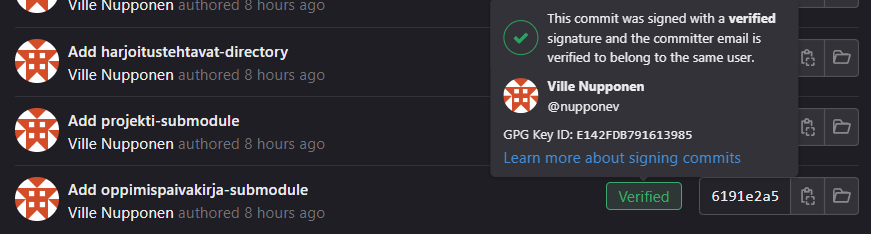
\includegraphics[width=\textwidth]{figures/gitlab-commit-verified.png}
    \caption{Kuvankaappaus Gitlabin commit listasta, jossa vahvistettu commitin allekirjoitus}
    \label{fig:gitlab-commit-verified}
\end{figure}

\begin{figure}[h!]
    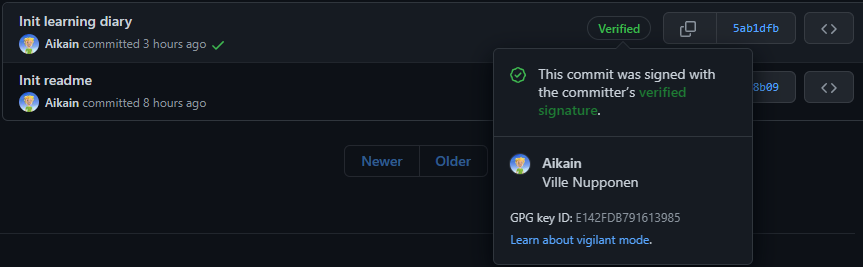
\includegraphics[width=\textwidth]{figures/github-commit-verified.png}
    \caption{Kuvankaappaus Githubin commit listasta, jossa vahvistettu commitin allekirjoitus}
    \label{fig:github-commit-verified}
\end{figure}

\section{Oppimispäiväkirja}

Oppimispäiväkirjan ohjeissa ohjeistettiin käyttämään pohjana opiskelijan
käsikirjasta löytyvää Diplomityö-ohjeessa \parencite{TuniIntraDiplomityo}
mainittua pohjaa. Ohjeista löytyy linkki Githubissa olevaan Ville Koljosen
tekemään LaTeX-pohjaan \parencite{GithubVillekolTauLatexThesisTemplate}.
Kyseinen pohja on vastaava kuin mitä käytin edellisenä vuonna kandidaationtyön
\parencite{GithubAikainCOMP200} tekemisessä.

Tämä oppimispäiväkirja on luotu kopioimalla kandidaation työn lopullinen
versio ja poistamalla kaikki sisältö. Tällöin saatiin itselle tutut asetukset
ja workflowt ilman, että tarvitsee niitä tehdä uudelleen. Pohjaa on muokattu
sen verran, että pohja ei vaadi tarkastajan kirjoittamista. Lisäksi viittaus
tapana käytetään numerointia eikä APA-merkintä tapaa. Tätä on kuitenkin
tarvittaessa helppo vaihtaa määrityksistä. Pohjassa numeeriset viittaukset
määriteltiin myös aakkosjärjestykseen kuten APA:ssa, mutta tämä johtui siitä,
ettei lähdeluettelon määrityksessä käytetty määriteltyä järjestystä.

\subsection{Kirjoittamiseen käytettävä IDE}

Kandidaatintyötä tehdessä käytössä oli Intellij IDEA ja siihen asennettuna
lisäosa, jotta saatiin tuki LaTeXille. Lisäksi koneelle asennettiin tuolloin
MiKTeX. Lisäosa ei kuitenkaan toiminut niin sujuvasti kuin olisi toivonut,
joten tällä kertaa päätin kokeilla mielestäni yksinkertaisemmalla tavalla eli
kevyemmällä IDE:llä ja terminaalilla.

Jetbrains julkaisi \parencite{JetbrainsFleetPublicPreview} 2022 lokakuussa
uuden Fleet-IDEn julkisen previewin, jonka myötä kyseistä IDEä on ollut
mahdollista käyttää ilman, että kuuluu suljettuun testiporukkaan. julkaisun
jälkeen olen itse ottanut käyttöön kaikkiin, joita varten ei selvästi ole
specifiä IDEä. Oppimispäiväkirja on pitkälti vain tekstiä, koodinpätkiä ja
kuvia, joten toimii täydellisesti siihen. Varsinaista tukea erityisesti
LaTeXille ei ole, mutta tämä ei ole merkittä muutos nähden aiempaan ratkaisuun,
jossa tuki oli hyvin olematon.

Fleet on siis jo parin kuukauden ajalta tuttu, joten se oli jo valmiina
asennettuna. Myös Fleetin navigointi ja pikanäppäimet ovat tutut ja tekevät
oppimispäiväkirjan työstämisestä LaTeXilla helpohkoa. UI on myös mukavan
minimalistinen, kuten kuvassa \ref{fig:fleet-ui} näkyy. Suurin puute on
automaattisen täytön puuttuminen, kun lisää uuden viittauksen lähteeseen,
mutta muuten ei ole aloittaessa ainakaan ilmennyt muita asioita, jotka
häiritsivät oppimispäiväkirjan tekemistä.

\begin{figure}[h!]
    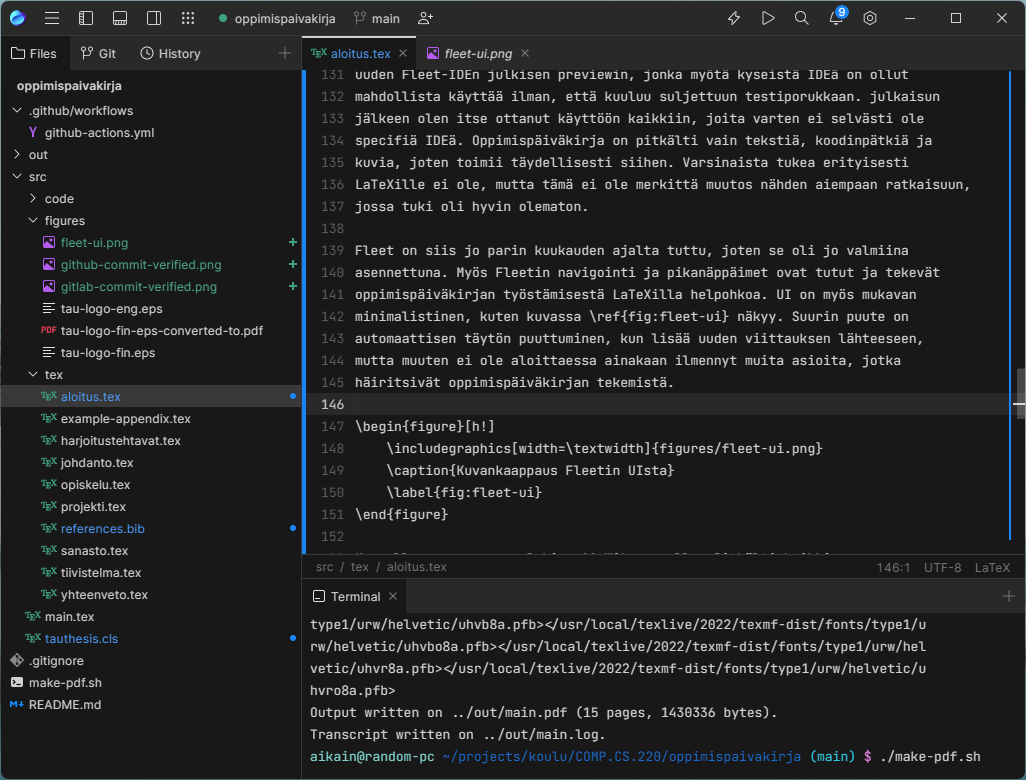
\includegraphics[width=\textwidth]{figures/fleet-ui.png}
    \caption{Kuvankaappaus Fleetin UI:sta}
    \label{fig:fleet-ui}
\end{figure}

\subsection{PDF:n generointi paikallisesti}

Koneelle on asennettu Debian 11 WSL:n avulla. Pitkälti kaikki
komentorivityökalut, joita käytän, on asennettu Debianille. Kaikki komennot,
joita tässä työssä käytetään, suoritetaan Debianin sisällä sen ollessa
luontevampaa ja kätevämpää kuin käyttää esim. cmd tai powershell. Lisäksi muut
ratkaisut, kuten cygwin, eivät ole onnistuneet osoittamaan toimivuutta yhtä
kattavasti.

Aiemmin LaTeXia käytettäessä tarvittavat ohjelmistot oli asennettu Windowsin
puolelle, joten siihen liittyvät oli nyt asennettava uudestaan. Debianin
käyttämästä pakettihallinnasta löytyi suoraan texlive-paketti, joka vaikutti
sisältävän kaiken tarvittavan, joten asennus vaikutti hyvin suoraviivaiselta:

\begin{lstlisting}[
    basicstyle=\small,
    label={lst:install-texlive},
    language=bash,
]
    # apt install texlive
\end{lstlisting}

Tämän jälkeen käytettävissä oli pdflatex-komento, jota käytetään PDF:n
generointiin. LaTeX-pohjassa löytyi valmiit ohjeet terminaali pohjaiseen
käyttöön:

\begin{lstlisting}[
    basicstyle=\small,
    label={lst:install-texlive},
    language=bash,
]
    $ pdflatex main.tex
    $ makeindex -s main.ist -t main.glg -o main.gls main.glo
    $ biber main
    $ pdflatex main.tex
    $ pdflatex main.tex
\end{lstlisting}

Kuitenkin jo ensimmäistä komentoa ajaessa ilmeni ongelmia. Komento ei
generoinut kaikkia tarvittavia tiedostoja, joita komento itse tarvitsi
myöhemmin. Lisäksi makeindex-komennon tarvitsevat main.ist- ja main.glo-
tiedosto puuttuivat. Näiden lisäksi myös biber-komentoa ei löytynyt sillä
kyseisen riippuvuutta ei saatu asennettua. pdflatex-komento varoitti lisäksi
vanhasta versioista ja ohjeisti päivittämään uuteen.

Saatuja ohjeita \parencite{TeXLiveQuickInstall} noudattaen texliven päivitys
onnistui vaivattomasti. Päivityksen jälkeen aiemmin ilmenneet ongelmat
katosivat ja ratkaistavana olivat vain yksittäiset syntaksivirheet sekä
yksi puuttuva riippuvuus. Riippuvuuksia saadaan asennettua tlmgr-komennolla.
Kyseinen komento vaatii kuitenkin ensimmäisellä kerralla alustuksen:

\begin{lstlisting}[
    basicstyle=\small,
    label={lst:init-tlmgr},
    language=bash,
]
    $ tlmgr init-usertree
\end{lstlisting}

jonka jälkeen puuttuva riippuvuus saatiin asennettua:

\begin{lstlisting}[
    basicstyle=\small,
    label={lst:init-tlmgr},
    language=bash,
]
    $ tlmgr install titlesec
\end{lstlisting}

PDF:n generointi aiemmin esiteltyhjen komentoje avulla generoi PDF:n lisäksi 16
muuta tiedostoa. Oletuksena nämä tiedostot sijoittuivat main.tex-tiedoston
kanssa samaan kansioon, joka teki oleellisista tiedostoista hankalampilöytyisiä
tiedostorakenteen kautta. Tämän seurauksena automaattisesti generoidut
tiedostot, joita ei sen myötä myöskään tarvitse lisätä versionhallintaa, olisi
kätevä saada omaan kansioonsa. Tämä onnistuu muutamalla lisäflagilla
komentoihin:

\begin{lstlisting}[
    basicstyle=\small,
    label={lst:init-tlmgr},
    language=bash,
]
    $ pdflatex -output-directory=../out main.tex
    $ biber --output-directory ../out main
\end{lstlisting}

makeindex-komento ei kuitenkaan vaikuttanut osaavan luoda tiedostoja muualla
kuin nykyiseen kansioon (tai sen alakansioihin), joten src-kansion ulkopuolella
oleva kansio ei suoraan onnistuisi. Tämä saadaan kuitenkin tehtyä vaihtamalla
kansiota kyseisen komennon ajaksi generoiduille tiedostoille luotuun kansioon.
Komentoja ollessa jo valmiiksi useita ja joiden lisäksi kansion vaihtamisia,
oli tähän kätevämpi luoda yksinkertainen bash-scripti \ref{lst:make-pdf}, joka
tekee kaiken tarvittavan.

\lstinputlisting[
    basicstyle=\small,
    caption={Bash-scripti PDF:n generointiin},
    label={lst:make-pdf},
]{code/make-pdf.sh}

Tämän jälkeen muutoksien jälkeen saadaan generoitua PDF paikallisesti:

\begin{lstlisting}[
    basicstyle=\small,
    label={lst:init-tlmgr},
    language=bash,
]
$ ~/projects/koulu/COMP.CS.220/oppimispaivakirja/make-pdf.sh
\end{lstlisting}

\subsection{PDF:n generointi automaattisesti}

Paikallisen generoinnin lisäksi PDF saadaan generoitua automaattisesti Github
Actioneiden avulla. Nämä on määritelty oppimispäiväkirjan repositoryssa
.github/workflows-kansiossa Github Action for LaTeX -actionin ohjeiden
\parencite{GithubActionsForLaTeX} mukaisesti. Määritykset saatiin suoraan
valmiiksi kopioitua kandidaationtyön repositorysta. Osasta actioneita oli
Kuitenkin tullut uudet versiot, joten ne päivitettiin uudempiin. Lisäksi
triggeröinti sääntöjä tarkennettiin, jotta PDF generoidaan vain jos sen
generointiin käytettävät tiedostot muuttuvat.

Kun muutokset commitataan ja pushataan, käynnistyy automaattisesti workflow,
joka on nähtävissä Githubissa repositoryn Actions-välilehdessä. Noin 2 minuutin
odottamisen jälkeen työ valmistuu ja ja artifakteista löytyy PDF.zip tiedosto
ladattavaksi, jonka sisältä löytyy generoitu main.pdf-tiedosto.

\subsection{Run-configuraatio Jetbrains Fleetiin}

Jetbrains Fleetiin on mahdollista määritellä Run Configuration, jonka avulla
voisi olla helpomi ajaa kuin pitää auki erillistä terminaalia, josta ajaa
komento aina eriskeen. Kuitenkaan tämän määritys ei lähtenyt toimimaan niin
yksinkertaisesti kuin olisi voinut toivoa, joten liian ajan käyttäminen ei
ole kannattavaa näin pienen asian suhteem.

\section{Android Studion asennus}

Jetbrainsin tuotteiden ollessa ennestään tuttuja ja aktiivisessa käytössä, on
käytössä myös Jetbrains Toolbox, joka mahdollistaa Jetbrainsin IDE:jen
asentamisen vaivatta. Tämän avulla onnistuu myös Android Studion asentaminen
yhdellä klikkaukselle.

Asennuksen yhteydessä ilmenee ongelma HAXM:n asentamisessa:

\begin{displayquote}
Intel® HAXM installation failed. To install Intel® HAXM follow the instructions found at: https://github.com/intel/haxm/wiki/Installation-Instructions-on-Windows
\end{displayquote}

Ongelma vaikuttaisi johtuvan Windowsin ytimen eristyksestä ja korjaantuisi se
pois kytkemällä \parencite{GithubIntelHaxmIssue412}. Kuitenkaan KAXM:n ollessa
vain parannus emulaattorin suorituskykyyn, ei ytimen eristyksen kytkeminen pois
päältä ole välttämättä kannattavaa.

Ensimmäisellä yrittämällä vaikuttaisi ettei projektin luonti toimi WSL:n
sisälle. Tähän tarkempaa perehtymistä harjoitus 3:n yhteydessä.

\section{Tuntikirjanpito}

Kurssin edetessä kirjaan tunnit niihin asioihin mihin kyseisestä asiasta
kirjoitettu teksti sisältyy oppimispäiväkirjassa. Lopullinen yhteenveto eri
osioiden yhteenlasketusta tuntikirjanpidosta löytyy yhteenvedosta.

Alla olevaan taulukkoon on kirjattu aloitukseen käytetyt tunnit. Näiden lisäksi
taulukkoon on laitettu ne tunnit, joissa on selvästi keskitytty
oppimispäiväkirjan tekemiseen niiltä osilta kun oppimispäiväkirjaa ei ole tehty
sujuvasti muun tekemisen ohessa tai on vaatinut asioiden siistiksi
kirjoittamista.

Käytetty aika on kirjattu 5min tarkkuudella. Tämä lähinnä, koska samaa käytäntöä
käyttää töissä ja helpoittaa hahmottamaan mitä asioita tehnyt ja milloin.

\begin{table}[H]
  \centering
  \label{tab:other-studing-working-hours}
  \begin{tabular*}{\linewidth}{@{\extracolsep{\fill}} l c c c r }
    \textbf{Tekeminen} & \textbf{Päivämäärä} & \textbf{Aloitettu} & \textbf{Lopetettu} & \textbf{Määrä} \\
    \hline
    Versionhallinnan alustus          & 19.01.2023 &     - &     - & 1h 00m \\
    Oppimispäiväkirjan alustus        & 19.01.2023 &     - &     - & 2h 00m \\
    Oppimispäiväkirjan kirjoittaminen & 20.01.2023 &     - &     - & 3h 00m \\
    Oppimispäiväkirjan kirjoittaminen & 23.05.2023 & 08:30 & 12:05 & 3h 35m \\
    Oppimispäiväkirjan kirjoittaminen & 29.05.2023 & 23:40 & 01:00 & 1h 20m \\
    Oppimispäiväkirjan kirjoittaminen & 30.05.2023 & 22:55 & 23:55 & 1h 00m \\
    Oppimispäiväkirjan kirjoittaminen & 31.05.2023 & 11:15 & 11:50 &    35m \\
    Oppimispäiväkirjan kirjoittaminen & 31.05.2023 & 13:00 & 13:20 &    20m \\
    Oppimispäiväkirjan kirjoittaminen & 31.05.2023 & 15:25 & 15:45 &    20m \\
    Oppimispäiväkirjan kirjoittaminen & 31.05.2023 & 22:30 & XX:XX & ?? \\
    \hline
    \multicolumn{4}{l}{\textbf{Yhteensä}} & \textbf{Xh XXm} \\
  \end{tabular*}
\end{table}


\chapter{OPISKELU}
\label{ch:opiskelu}
Tähän tulee tietoa miten kurssin asioita opiskeltiin kurssin edetessä yms.


\chapter{HARJOITUSTEHTÄVÄT}
\label{ch:harjoitustehtavat}
% TODO START

Tähän tulee tietoa kurssin harjoitustehtävien tekemisestä.

% TODO END

\section{Harjoitus 1}

% TODO START

Tavoitteena selvittää jonkin mobiililaitteen ohjelmointiin vaadittavat asiat.

* Valitse laite joka kiinnostaa( esimerkiksi oma puhelin tai tabletti)

* Merkki, mallii?

* Selvitä laitteen käyttöjärjestelmä versio ja ominaisuudet. (Linkki valmistajan esitteeseen?)

* Selvitä mahdolliset ohjelmointi kielet.

* Selvitä ohjelmointiin tarvittavat työkalut ( + käyttöjärjestelmät?)

* Sisältääkö laite valmistajakohtaisia sovelluksia tai ominaisuuksia? Ja mitä tarkoitetaan (mainos)termillä ”puhdas Android”?

* ”App Store” (laitteen / valmistajan) – onko sinne mahdollista saada itsekoodattu sovellus?

* Selvitä laitteesta löytyvät ominaisuudet (esim GPS) ja pystytäänkö niitä käyttämään alustan tarjoamilla ohjelmointikielillä.

Tavoitteena noin sivun mittainen selvitys, jossa viittauksia lähteisiin. Kaikkia tietoja ei
tarvitse kirjata vaan lähteiden viitteitä voi käyttää apuna(esimerkkinä puhelimen
ominaisuuksia ei kannata kaikkia kirjata)

% TODO END

\section{Harjoitus 2}

Versionhallinnan käyttö on tullut aloitettua lähes 10 vuotta sitten ja on
välttämätön työkalua niin töissä, opiskelussa kuin vapaa-ajan projekteissakin,
joten uskon käytön vähintään peruskäytön hallitsevan. Tämän vuoksi erillistä
harjoitus ohjeen mukaista harjoitus2\_vastaus.txt-tiedostoa ei ole lisätty.

Käytössä on lisäksi ssh-avaimet, kuten harjoituksessa viitattiin. Näiden
lisäksi myös commitit allekirjoitetaan ja käytössä submoduuleja. Näistä oli
tarkemmin selitystä aloitus-osiossa.

Oppimispäiväkirja on myös versionhallinnassa ja PDF-muoto siitä generoidaankin
automaattisesti Github Actioneilla, jotka ovat merkittävä apu asioiden
automatisoinnissa kätevästi versionhallinnan kanssa.

\section{Harjoitus 3}

Android Studion asentamisesa on kerrottu tarkemmin aloitus-osiossa.

Oppimispäiväkirja-repository ja sen myötä myös harjoituksien kansiot
sijaisevat WSL:n tiedostojärjestelmässä. Tähän on keino päästä käsiksi kuten
mm. verkkojakoihin, toisiin kovalevyihin yms. Android Studio ei kuitenkaan
toimi tämän kautta vaan näyttää \ref{fig:android-studio-path-not-writable}
mukaisen virheen, ettei kansio ole kirjoitusoikeuksia.

\begin{figure}[h!]
    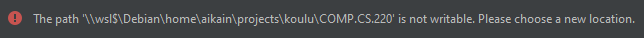
\includegraphics[width=\textwidth]{figures/android-studio-path-not-writable.png}
    \caption{Kuvankaappaus Android Studio virheestä kirjoittaa kansioon}
    \label{fig:android-studio-path-not-writable}
\end{figure}

Projektin voi kuitenkin luoda muutoin WSL:n puolelle ja sen jälkeen avata
Android Studiolla. Tästä kuitenkin aiheutuu uusi ongelma; Gradle ei saa
syncattua haluamiaan asioita vaan sanoo ''virhe, yritä uudelleen'' tarkentamatta
mikä virhe. Logeista löytyy hiukan tarkempi virhe:

\begin{displayquote}
GradleConnectionException: Operation result has not been received
\end{displayquote}

Tämän virheen perusteella ei kuitenkaan löydy mitään Android Studioon itseensä
liittyvää vaan kaikki viittaavat kahteen Intellij IDEAn issueeseen (joka toki
tässä tapauksessa on tarpeeksi lähellä), mutta molemmissa puhutaan Android-
lisäosan kytkemisestä pois päältä ja se ei oikein toimi ratkaisuna tähän
tilanteeseen.

On hyvin mahdollista, että virhe johtuu SDK:n sijaitsemisesta Windowsin
puolella kun kaikki muut (projekti, gradle, jdk) sijaisevat WSL:n sisällä.
Kuitenkin kokemuksen pohjalta yleensä fyysisten laitteiden kanssa kommunikointi
WSL:n sisältä käsin on hyvin nihkeää ja jo emulaattorinkin käyttö saattaisi
tuottaa ongelmia, joten ei ole mielekästä lähteä asentamaan Android SDK:ta ja
kaikkea siihen liittyvää WSL:n sisälle.

Pitkälti siis ainut toimiva ja aikaa säästävä ratkaisu on pitää projektit
Windowsin puolella. Kuitenkaan yksittäisten projektin vuoksi en ole siirtämässä
versionhallintaa ja kaikkea muuta configuraatiota toimimaan WSL:n ulkopuolella,
joten tarvitaan keino pitää repo WSL:ssä, mutta harjoitustehtävät Windowsin
puolella. Ensimmäisenä tähän tulee mielenä yksinkertaisesti käyttää symboolista
linkkiä.

\begin{lstlisting}[
    basicstyle=\small,
    label={lst:symbolic-link-harjoitustehtavat},
    language=bash,
]
    # ln -s /mnt/c/Users/Aikain/AndroidStudioProjects/mobiiliohjelmointi-kurssi-harjoitustehtavat/ harjoitustehtavat
\end{lstlisting}

Symboolin linkki näkyy kuitenkin Gitille symboolisena linkkinä eikä normaaleina
tiedostoina, mikä toki on täysin perusteltua mm. tietoturvasyistä. Puolestaan
ns. kovan linkin tekeminen ei ole mahdollista kansioille. Vaihtoehtoisesti
voisi kokeilla linkin tekemistä toisinpäin
\parencite{StackoverflowWSLSymlink}.

\begin{lstlisting}[
    basicstyle=\small,
    label={lst:powershell-link-harjoitustehtavat},
    language=PowerShell,
]
    New-Item -ItemType SymbolicLink -Path ''C:\Aikain\Users\AndroidStudioProjects\mobiiliohjelmointi-harjoitustehtavat'' -Target ''\\wsl$\Debian\home\aikain\projects\COMP.CS.220\harjoitustehtavat''
\end{lstlisting}

Tämä kuitenkin aiheuttaa jälleen samat ongelmat kuin aiemmin Android Studion
kanssa kun yritti käyttää suoraan WSL:n sisällä olevaa sijaintia.

Ei ehkä niin hyvänä ratkaisuna, mutta kuitenkin toistaiseksi toimiva ratkaisu
saadaan käyttämällä bind mountia \parencite{BaeldungBindMounts}.

\begin{lstlisting}[
    basicstyle=\small,
    label={lst:bind-mount-harjoitustehtavat},
    language=bash,
]
    $ mount -o bind /mnt/c/Users/Aikain/AndroidStudioProjects/mobiiliohjelmointi-harjoitustehtavat /home/aikain/projects/koulu/COMP.CS.220/harjoitustehtavat
\end{lstlisting}

Versionhallintaan lisätessä kiinnitin huomiota tarkemmin noihin gradle
tiedostoihin. Jotenkin olen sitä vastaan, että jar-tiedoston laittaisi
versionhallintaan, mutta Gradlen dokumentaatiossa
\parencite{GradleDocsGradleWrapper} sanotaan seuraavasti:

\begin{displayquote}
To make the Wrapper files available to other developers and execution
environments you’ll need to check them into version control. All Wrapper files
including the JAR file are very small in size. Adding the JAR file to version
control is expected. Some organizations do not allow projects to submit binary
files to version control. At the moment there are no alternative options to the
approach.
\end{displayquote}

Toistaiseksi siis laittelen nämä versionhallintaan, mutta olisi hyvä jos tähän
olisi parempi ratkaisu.

Lisäksi .idea-kansion sisältö ei ole oletuksena kokonaan .gitignore:ssa.
Ilmeisesti toki pääosa käyttäjistä käyttää Android Studio:ta, mutta silti IDEn
configuraation laittaminen versionhallintaan ei tunnu oikealta ratkaisulta,
varsinkin kun Android Studio osaa avata projektin ilman niitä ja mitään
projektille merkittäviä asioita ei pitäisi olla IDEn configuraatiossa, jotta
muunmuassa CI/CD toimii ongelmitta kun lähtökohtaisesti ne eivät ole tietoisia
IDEn confeista.

\section{Harjoitus 4}

Tarkoitus painottaa Kotlinilla tekemistä ja tehdä varsinkin projekti
Kotlinilla, joten tässäkin valittu pienempi eli harjoitus 4 javalla tehtäväksi
ja suurempi eli harjoitus 5 Kotlinilla tehtäväksi.

Painotus opiskelussa on ollut Composessa, jota puolestaan ei voi käyttää Javan
kanssa \parencite{StackoverflowComposeInJava}, joten alkuun pääseminen vaatii
muutaman minuutin mietintä tauon, mutta onneksi Android Studio alustaa
valmiiksi uuden projektin luonnin yhteydessä tarvittavat asiat.

\begin{wrapfigure}{r}{0.4\textwidth}
    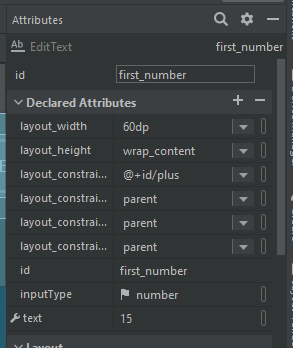
\includegraphics[width=0.4\textwidth]{figures/exercise-4-attributes.png}
    \caption{Kuvankaappaus Android Studio Design-työkalun attribuuteista}
    \label{fig:exercise-4-attributes}
\end{wrapfigure}

Design-työkalun avulla saa lisättyä helposti tarvittavat osat, mutta jotenkin
graaffisen käyttöliittymän kautta kuvassa \ref{fig:exercise-4-attributes}
näkyvien tietojen täyttäminen ei suju, joten aika vaihtaa Split-tilaan ja
muokata XML:ää suoraan. Tämä sujuukin suoraan helpommin ja jopa yleensä
päänvaivaa aiheuttavat app:layout\_constraintX\_toXOf -asetukset menevät
sujuvasti tällä kertaa.

Aluksi lisään kentät suoraan valmiina olevaan ConstraintLayout:in alle, mutta
tästä aiheutuu se etteivät ne ole nätisti tasattuna yhteen riviin vaan
painikkeen ollessa korkeampi on sen keskikohta selvästi alempana kuin muilla.
Tämän voisi sinääli korjata vain nopeasti marginilla, joka tuntuu huonolta
ratkaisulta. Hetken pohdinnan jälkeen saankin laitettua toisen
ConstraintLayout:in, jonka korkeus on vain sisällön verran ja saan sisällön
keskitettyä pystysuunnassa kyseisen komponentin suhteen. Hiukan paddingia
ConstraintLayout:lle ja numerokentille leveydet niin saadaan siististi yhteen
riviin tasaisin välein kuvan \ref{fig:exercise-4-constraint-layout} mukaisesti.

\begin{figure}[h!]
    \centering
    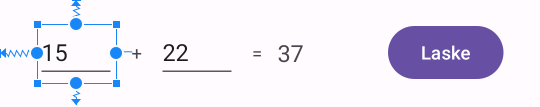
\includegraphics[width=0.8\textwidth]{figures/exercise-4-constraint-layout.png}
    \caption{Kuvankaappaus komponenttien sijoittelusta}
    \label{fig:exercise-4-constraint-layout}
\end{figure}

UI:n tultua valmiiksi viewBinding-ominaisuuden enablointi ja sen jälkeen
saadaankin helposti lisättyä painikkeelle onClickListener, joka ottaa kentistä
luvut ja laskee ne yhteen ja laittaa tulos-kenttään.

\begin{wrapfigure}{rl}{0.3\textwidth}
    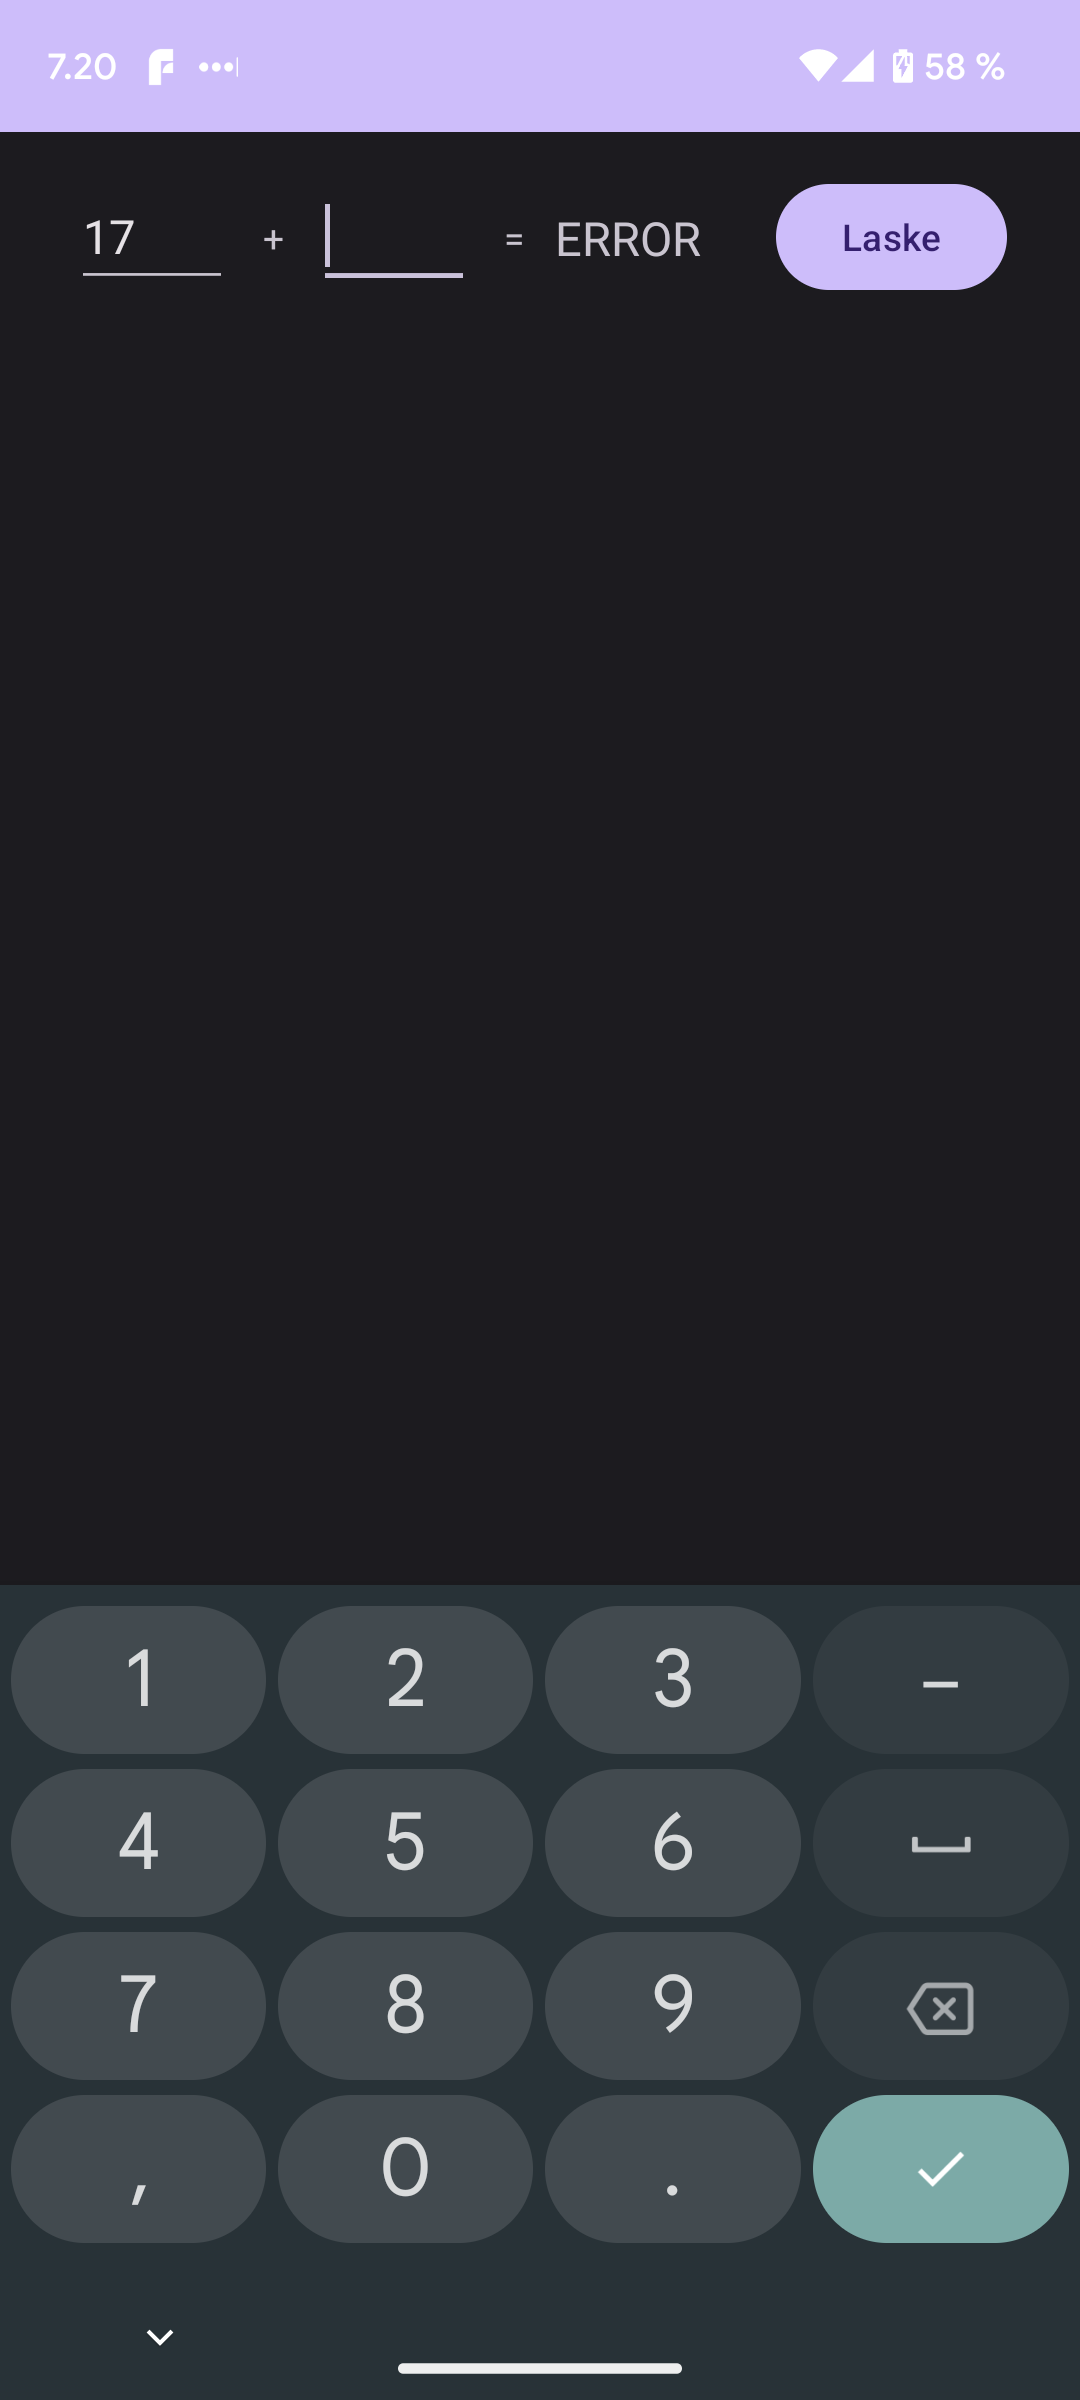
\includegraphics[width=0.3\textwidth]{figures/exercise-4-final.png}
    \caption{Kuvankaappaus lopullisesta sovelluksesta puhelimessa}
    \label{fig:exercise-4-final}
\end{wrapfigure}

Lopulta emulaattorissa toimisen jälkeen vielä hyvä hetki kokeilla, että toimii
sujuvasti puhelimellakin kuten kuvassa \ref{fig:exercise-4-final} näkyy.

Android Studio auttaa vielä nopeasti poistamaan tekstien kovakoodaukset ja
käyttämään strings-resursseja. Parannettavaa näinkin piennessä sovelluksessa
olisi vielä mm. saavutettavuuden suhteen sekä automaattisten testien
tekemisessä. Toki parannettavaa löytyy aina, joten jätetään sovellus tämän
harjoituksen osalta tähän.

\tipbox{
\textbf{Miksi packagen nimen alkuun in.aika?}

Harjoituksissa ja projekteissa esiintyy in.aika-verkkotunnusta. Tämä voi
vaikuttaa hiukan oudolta aluksi, että käytössä Intialainen verkkotunnus. Tähän
on kuitenkin yksinkertainen selitys. Olen pitkään käyttänyt nimimerkkiä
"Aikain" ja kuten jokaisella ''IT-nörtillä'' niin pitäähän minullakin olla
omaverkkotunnus (tai tänä päivänä niitä on jo useita..). Harmikseni aikain.fi
oli varattu, mutta aika.in-verkkotunnus puolestaan oli juuri sopivasti
vapautunut, joten se on ollut nyt 6 vuotta minulla ja näkyy monessa
henkilökohtaisessa projektissani yms.
}

\section{Harjoitus 5}

Edellinen harjoitus tuli tehtyä javalla, joten tässä harjoituksessa Kotlinin
vuoro. Tarkoituksena myös käyttää Jetback Composea tässä ja myöhemmissäkin
vaiheissa sekä projektissa.

Composen tarjoaman esikatselun avulla saadaan nopsaan hahmoteltua laskimen
perusrivi, kuten kuvassa \ref{fig:exercise-5-row-preview}.

\begin{figure}[h!]
    \centering
    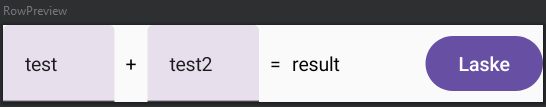
\includegraphics[width=0.8\textwidth]{figures/exercise-5-row-preview.png}
    \caption{Yhden laskurin rivin esikatselu}
    \label{fig:exercise-5-row-preview}
\end{figure}

Kun laskuoperaation merkki annetaan Composablelle parametrina, on koko laskimen
muodostaminen hyvin suoraviivaista UIn puolesta, kuten koodista
\ref{lst:full-calculator} ja kuvasta \ref{fig:exercise-5-calculator-preview}
nähdään.

\begin{lstlisting}[
    basicstyle=\small,
    label={lst:full-calculator},
    caption={CalculatorScreen-koodin hahmottelua},
    language=Kotlin,
]
@Composable
fun CalculatorScreen(
    modifier: Modifier = Modifier,
) {
    Column(modifier = modifier) {
        CalculatorRow(operator = "+")
        CalculatorRow(operator = "-")
        CalculatorRow(operator = "x")
        CalculatorRow(operator = "/")
    }
}
\end{lstlisting}

\begin{figure}[h!]
    \centering
    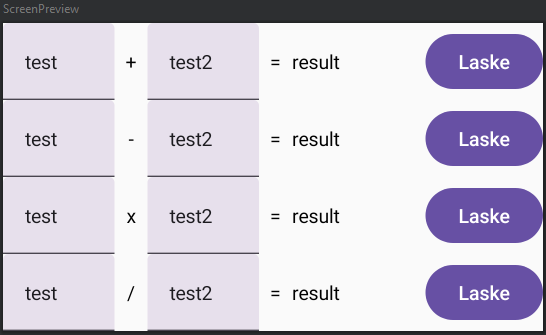
\includegraphics[width=0.8\textwidth]{figures/exercise-5-calculator-preview.png}
    \caption{Oheisen CalculatorScreen-koodin tuottama esikatselu}
    \label{fig:exercise-5-calculator-preview}
\end{figure}

Sovellukseen haluttiin toinen näkymä. Yksinkertaisuuden vuoksi lisätään näkymään
vain normaali painike ja painikkeen alle lista tehdyistä laskutehtävistä. Näkymä
saadaan nopeasti hahmoteltua ja esikatselua kuvassa
\ref{fig:exercise-5-history-preview} näkyvästä esikatselusta

\begin{figure}[h!]
    \centering
    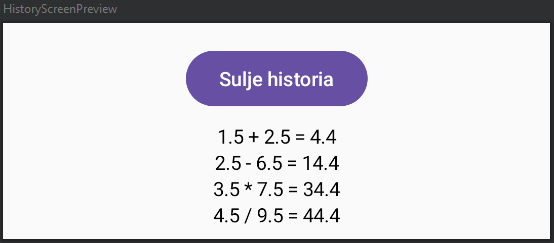
\includegraphics[width=0.8\textwidth]{figures/exercise-5-history-preview.png}
    \caption{Historianäkymän esikatselu}
    \label{fig:exercise-5-history-preview}
\end{figure}

Näkymien oltua karkeasti valmiina, on aika toteuttaa varsinainen
toiminnallisuus. Laskutoiminnallisuus saadaan yksinkertaisesti lisäämällä
riveille parametriksi funktio, joka hoitaa laskemisen. Tämän jälkeen riville
pitää vain toteuttaa Laske-painikkeelle käsittelijä, joka parsii rivillä
olevien kenttien numerot ja välittää ne parametrina saadulle lasku funktiolle,
jos numerot ovat kelvollisia. Mikäli numeron parsiminen ei onnistu tai lasku
funktio palauttaa null:in (vain jos yritetää jakaa nollalla), näytetään
käyttäjälle "ERROR"-teksti tuloksen sijaan. Jos puolestaan edes toinen kentistä
on tyhjä niin tyhjennetään tulosteksti.

Numeroiden parsiminen on sinääli haastava tehdä ilman ongelmia jo mm. eri
välimerkkien takia. Tämän huomaa hyvin kun saa sovelluksen kaatumaan useamman
kerran kun käyttää pilkkua pisteen sijaan. Try-catch parsimisen ja laskennan
ympärille ja käyttäjälle näkyviin "ERROR" muissakin virhetilanteissa niin
estetään sovelluksen kaatuminen. Mahdollisesti käyttämällä NumberFormat tms.
luokkaa voitaisiin parsiminen hoitaa perustuen Localeen, jolloin pilkut
voisivat toimia pisteen sijaan, mutta jotta asia pidetään yksinkertaisena,
käytetään vain valmista toDoubleOrNull-funktiota.

Seuraavaksi olisi laskujen tallentamisen vuoro ja ohjeessa sanotaan, että se
voidaan toteuttaa tavallisena tiedostoon kirjoituksena eikä tietokantaa
kannattaisi tähän rakentaa. Jääräpäänä en suostu tietoja tallentamaan
tiedostoon ellei ole ihan välttämätöntä kun liian monta kertaa törmännyt
projektiin, jossa on todettu ettei tietokantaa tarvitsisi vaikka oikeasti
tarvitsee ja joutunut näkemään ylimääräistä vaivaa sen vuoksi. Toki näin
harjoitustehtävässä, johon kukaan ei tule enää ikinä koskemaan, ei kyseistä
tilannetta tule tapahtumaan. Kuitenkin tehtävän annoin muotoilu antaa ymmärtää,
ettei tietokantaa tulisi käyttää sen aiheuttaman ylimääräisen vaivan vuoksi,
eikä niinkään sen vuoksi, että opettelisi kirjoittamaan tiedostoihin. Siispä
pitääkseni harjoituksen yksinkertaisena, käytän tietokantaa sen ollessa
huomattavasti nopeampaa ja yksinkertaisempaa toteuttaa kuin lähteä tutkimaan
miten tiedostoihin kirjoittaminen/lukeminen tapahtuu.

Tietokannan määrittämisessä toki onnistui pari huolimattomuutta tapahtumaan,
jonka seurauksena törmäsi käännösvirheeseen, joka johtui puuttuvasti
riippuvuudesta. Tämän lisäksi unohtui määrittää ID generoitumaan
automaattisesti, joten käytössä olleella IGNORE-käytönnöllä seurasi se, että
vain ensimmäinen tallentui tietokantaan. Kannan rakenteen muuttamisen jälkeen
sovellus kaatui vielä kerran kun unohtui muuttaa kannan versiota. Ilmeentyneet
ongelmat pieniä ja korjaantuivat kaikki helposti virheen perusteella ilman
tarkempaa tutkimista.

Hiukan UI:n tyylien säätämisen jälkeen sovellus onkin valmis käytettäväksi.
Käytettävyyttä saadaan parannettua, kun aktivoidaan numeronäppäimistö kenttiin
normaalin näppäimistön sijaan. Lisäksi historia näkymään lisätään scrollattava
lista, joka tukee suuria määriä tuloksia (LazyColumn). Vaihdetaan myös tehtyjen
laskujen järjestys käänteiseksi eli uusin ylimmäiseksi. Lopullisen sovelluksen
näkee kuvista \ref{fig:exercise-5-final-1} ja \ref{fig:exercise-5-final-2}.

\begin{figure}[h!]
\centering
\begin{minipage}[b]{.4\textwidth}
    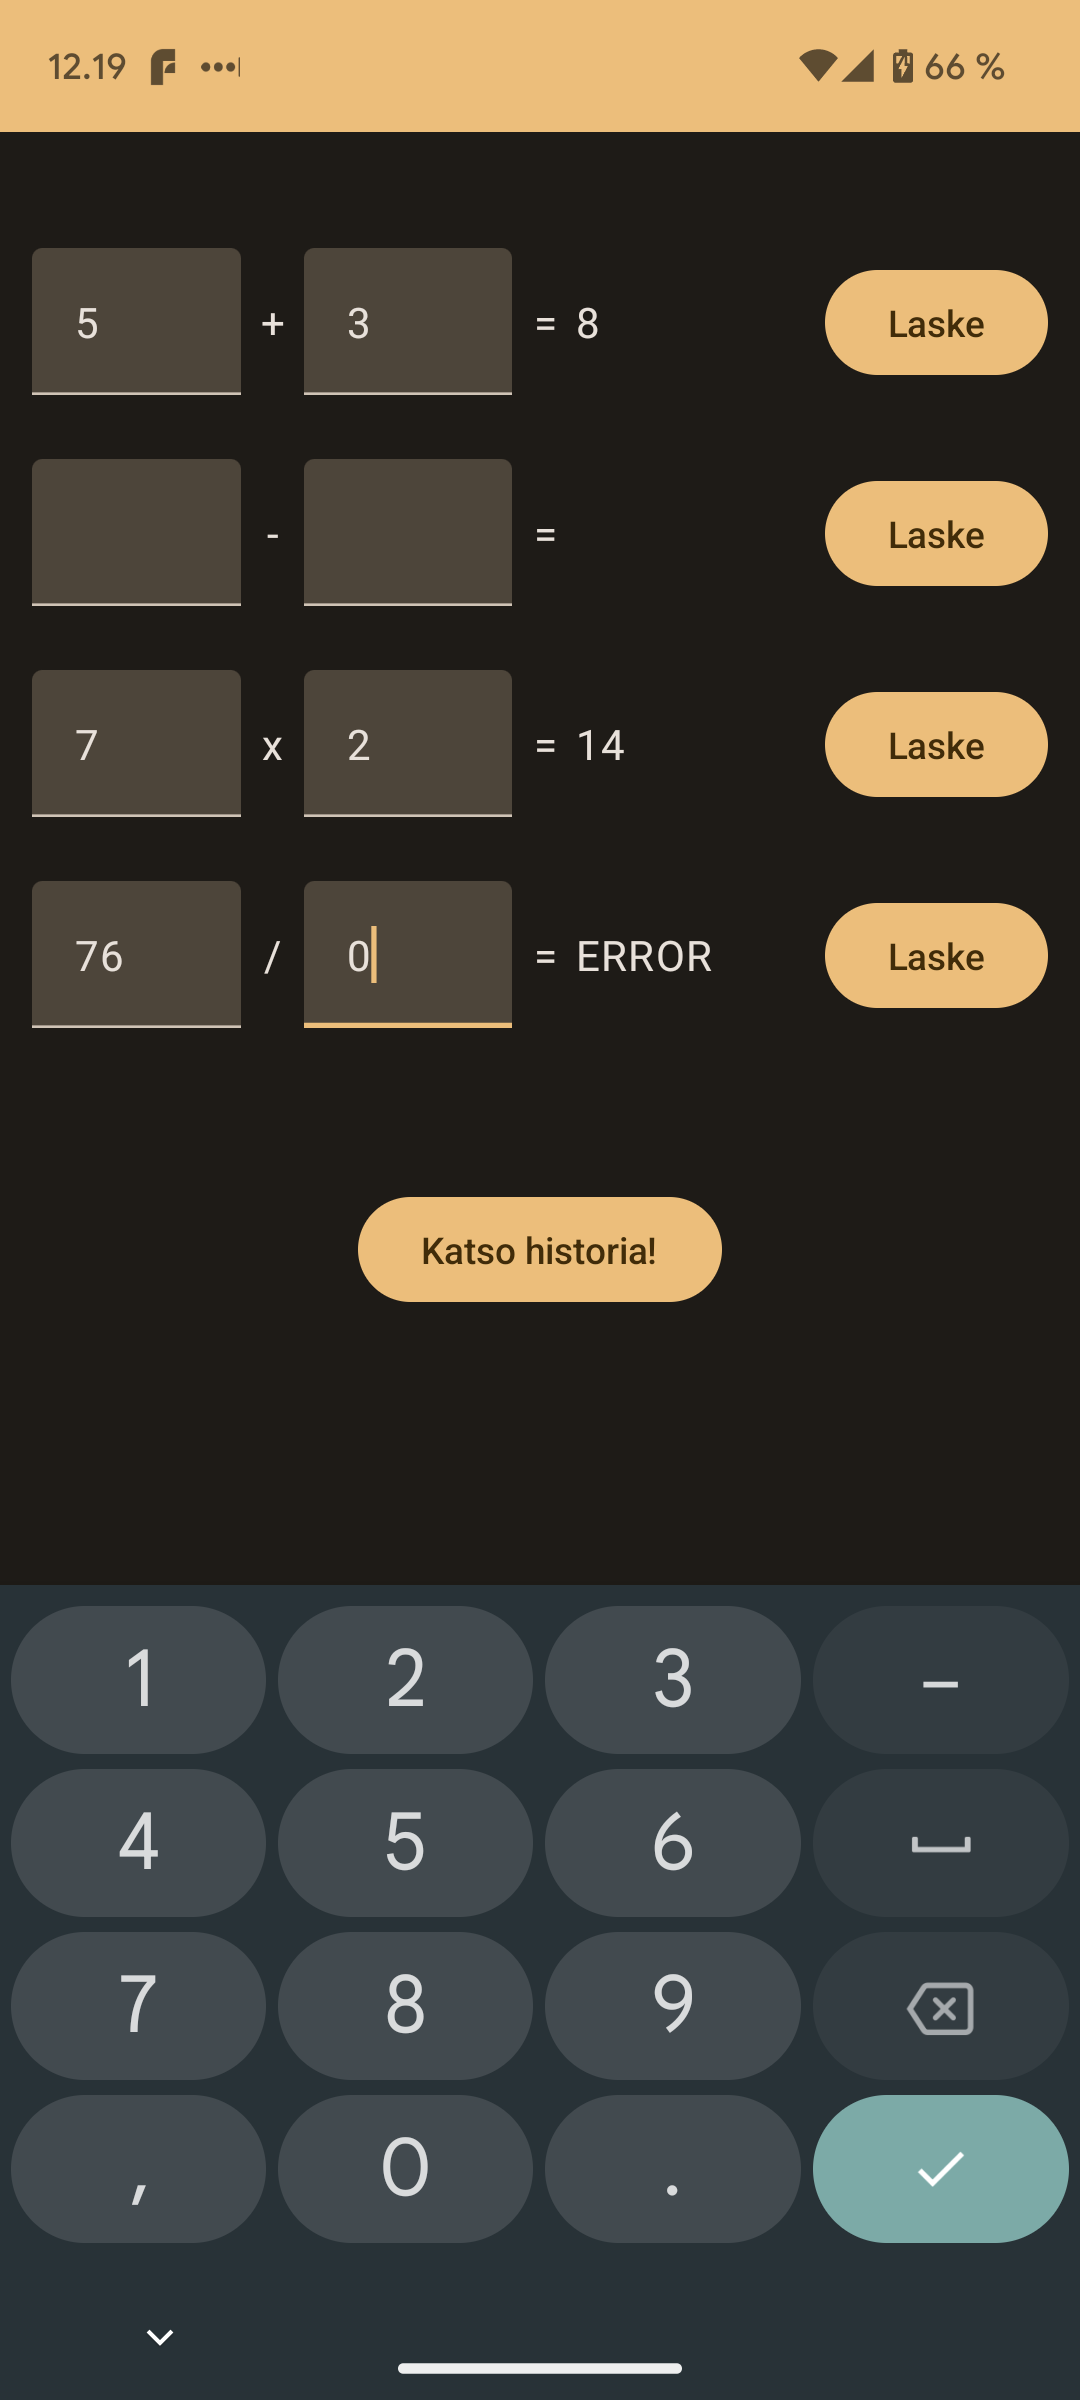
\includegraphics[width=\textwidth]{figures/exercise-5-final-1.png}
    \caption{Laskin näkymä}
    \label{fig:exercise-5-final-1}
\end{minipage}\qquad
\begin{minipage}[b]{.4\textwidth}
    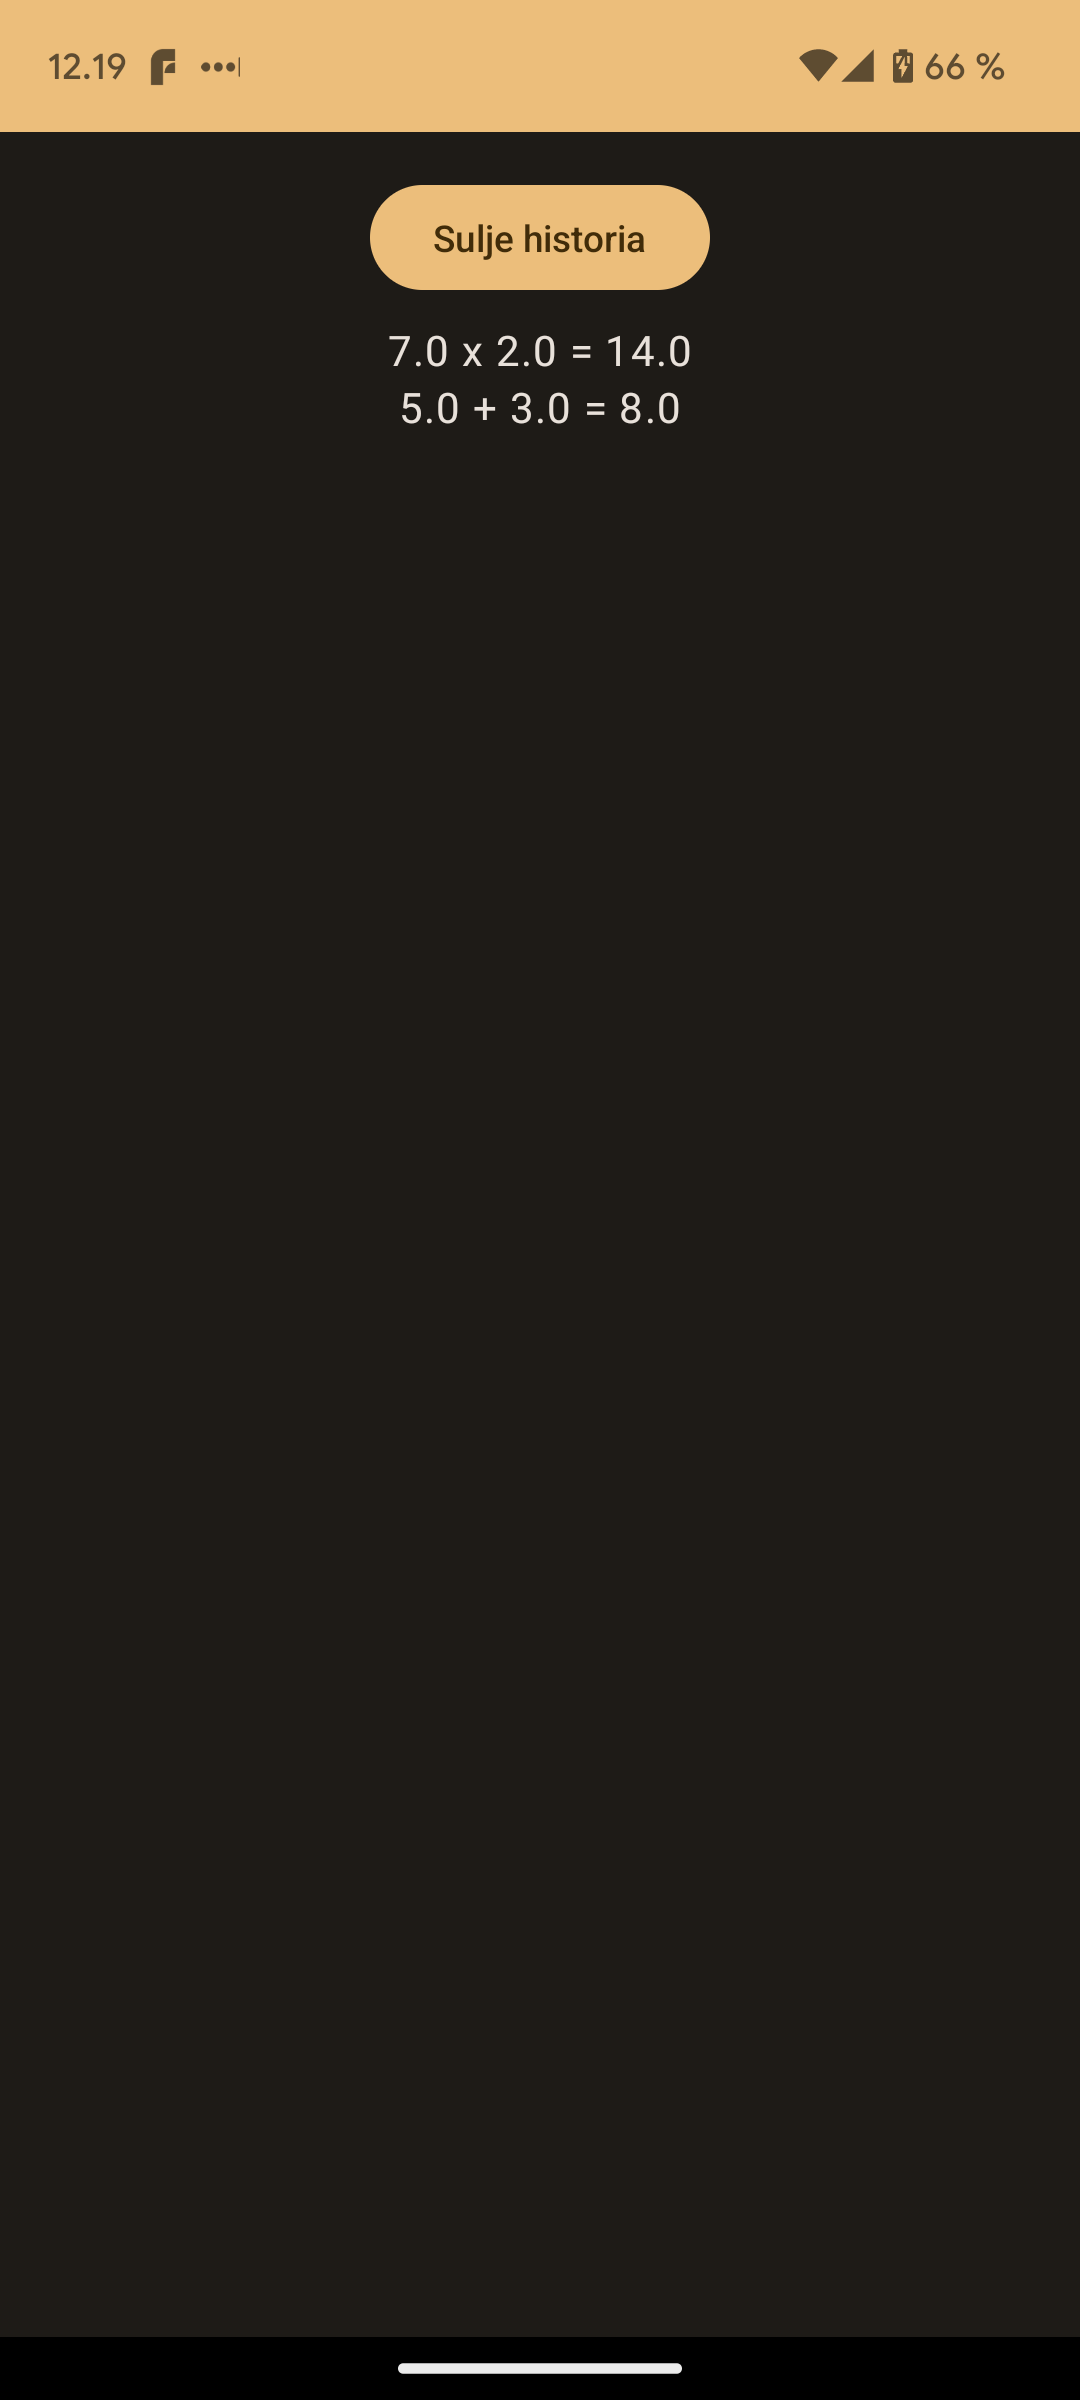
\includegraphics[width=\textwidth]{figures/exercise-5-final-2.png}
    \caption{Historia näkymä}
    \label{fig:exercise-5-final-2}
\end{minipage}
\end{figure}

Parannettavaa löytyy toki yhä tähänkin, mm. voisi käyttää repositoryja eikä
suoraan kutsua dao:a. Saavutettavuus kaipaisi tässäkin parantamista kuten myös
testejä. Nämä kaksi puutetta tulevat tosin todennäköisesti jatkuvaan jokaisen
harjoitustehtävän kohdalla.

Tämän harjoituksen tekemiseen tuli katseltua esimerkkiä Googlen kurssin
harjoitustehtävistä Inventory App \parencite{GithubGoogleDevTrainingInventory},
Bus Schedule \parencite{GithubGoogleDevTrainingBusSchedule}, Cupcake
\parencite{GithubGoogleDevTrainingCupcake} ja Unscramble
\parencite{GithubGoogleDevTrainingUnscramble}.

\section{Harjoitus 6}

Harjoituksen aiheeksi valittu paikan tallentaminen. Tietokantaan määritelty
neljä kenttää yksilöivän tunnisteen lisäksi kuten koodista
\ref{lst:location-data-class} on nähtävissä.

\begin{lstlisting}[
    basicstyle=\small,
    label={lst:location-data-class},
    caption={Location data class},
    language=Kotlin,
]
@Entity(tableName = "location")
data class Location(
    @PrimaryKey(autoGenerate = true)
    val id: Long = 0,

    val longitude: Double,
    val latitude: Double,
    val timestamp: Long,
    val notes: String,
)
\end{lstlisting}

Koska harjoituksessa painotuksena nimenomaan tietokanta ja sinne tiedon
tallentaminen, toteutan ensin tietokanta puolen ja vasta sen jälkeen lähden
hahmottelemenaan käyttöliittymää. Koska tietokanta tuli toteutettua jo
edellisessä harjoituksessa, menee sen toteuttaminen hyvinkin suoraviivaisesti.
Kuitenkin vastaan tulee aluksi ongelma, ettei Room tue OffsetDateTime-tyyppiä,
joten joko pitäisi rakentaa convertteri muuttamaan se sopivampaan muotoon tai
tyytyä siihen, että tallennetaan ajanhetki UNIX-aikana, poikkeuksena kuitenkin,
että käytetään millisekunteja sekuntien sijaan.

Tämän jälkeen listanäkymän hahmoittelu tiedoille, kuten esikatselussa
\ref{fig:exercise-6-location-screen} näkyy. Pari material iconia tietojen
kanssa niin ulkoasu näyttää merkittävästi paremmalta vaikka onkin hyvin
pelkistetty ilman tyylittelyä.

\begin{figure}[h!]
    \centering
    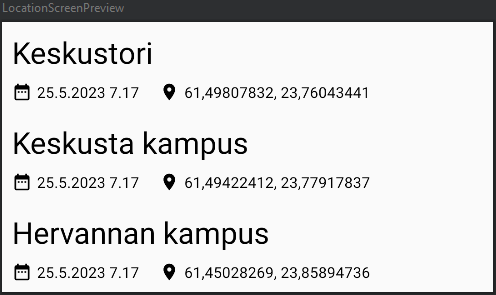
\includegraphics[width=0.8\textwidth]{figures/exercise-6-location-screen.png}
    \caption{Sijaintien listanäkymän esikatselu}
    \label{fig:exercise-6-location-screen}
\end{figure}

Haluan erotella tietojen lisäämisen perusnäkymästä, mutta täysin oman näkymän
tekeminen tuntuu myös vähän "tylsältä" ratkaisulta. Mahdollisesti dialogi tms.
voisi olla sellainen minkä haluaisin. Pienen Googlailun jälkeen mitä eri
komponentteja on saatavilla, törmään Material Designissa oleviin Bottom
Sheetseihin \parencite{MaterialComponentsBottomSheets}, jotka vaikuttavat
siistiltä ratkaisulta, vaikka niiden tarkoitus onkin ilmeisesti olla hiukan
enemmän lisätoiminnoille ja -sisällölle kuin niinkään uuden asian lisäämiseksi.
En ole kuitenkaan koskaan noita käyttänyt, joten aika kokeilla. Nopeahko
kuvan \ref{fig:exercise-6-location-insert-screen} mukainen hahmotelma
käyttöliittymälle, jonka jälkeen aika luoda ViewModelit ja yhdistää niiden
avulla data ja käyttöliittymä.

\begin{figure}[!ht]
    \centering
    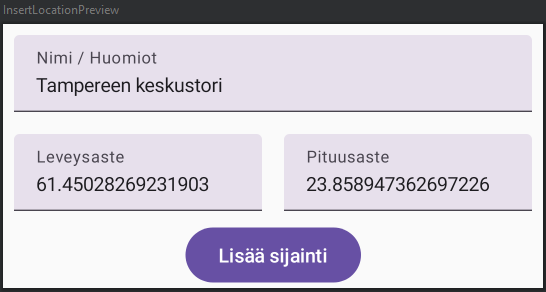
\includegraphics[width=0.8\textwidth]{figures/exercise-6-location-insert-screen.png}
    \caption{Sijaintien lisäys lomakkeen esikatselu}
    \label{fig:exercise-6-location-insert-screen}
\end{figure}

\begin{wrapfigure}{r}{0.3\textwidth}
    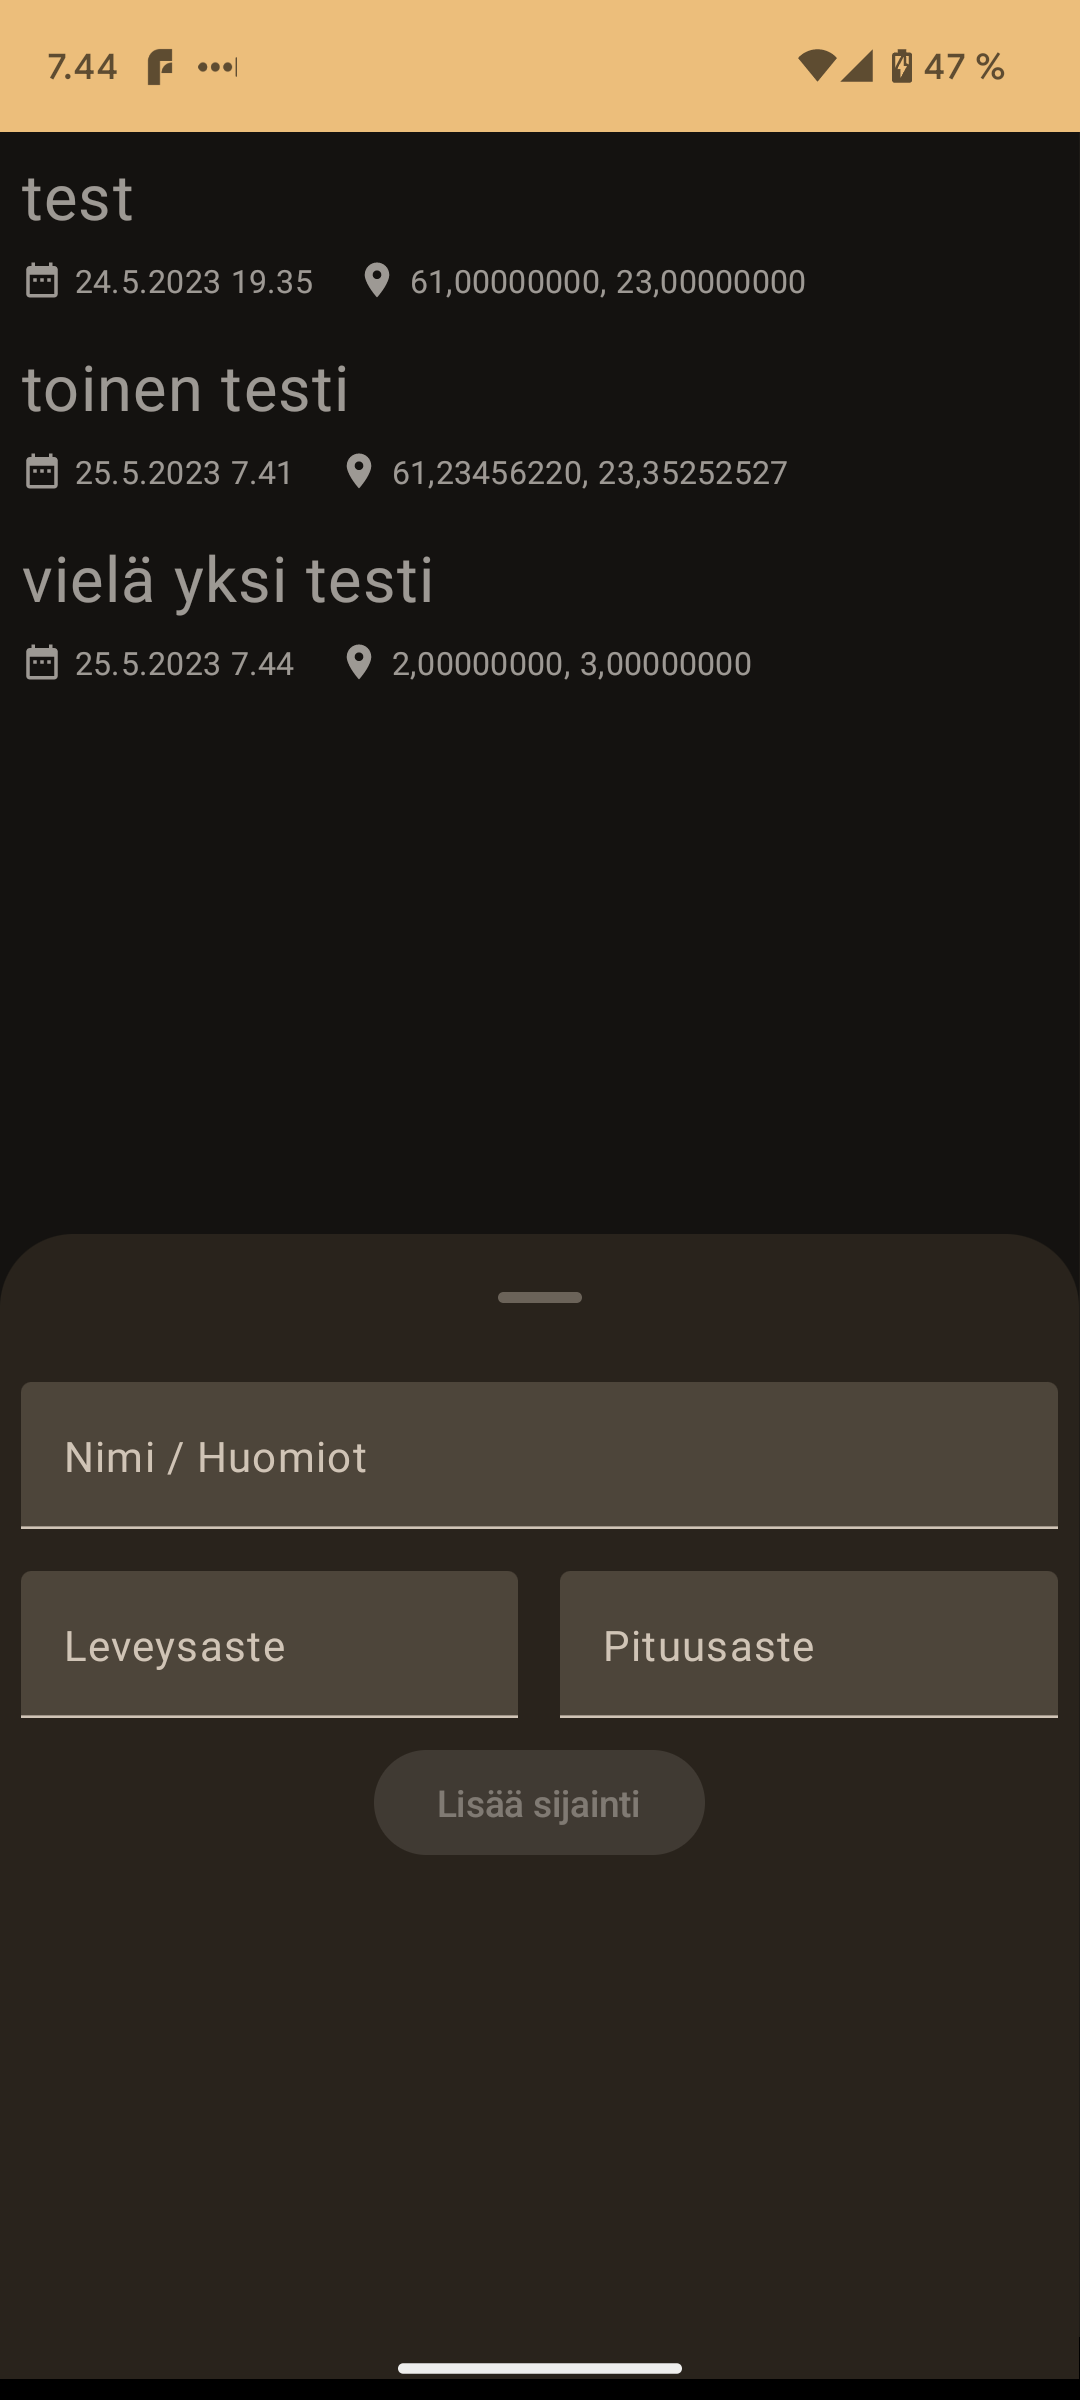
\includegraphics[width=0.3\textwidth]{figures/exercise-6-final.png}
    \caption{Kuvankaappaus lopullisesta sovelluksesta puhelimessa}
    \label{fig:exercise-6-final}
\end{wrapfigure}

Hiukan testailua puhelimella niin huomaa kaksi käytettävyyteen parannettavaa
asiaa: tekstikenttiihin hyvä lisätä labelit, jotka näkyvätkin jo kuvassa
\ref{fig:exercise-6-location-insert-screen}. Lisäksi tiedon lisäämisen jälkeen
käyttäjälle mukavampaa, jos vanhat tiedot tyhjennetty kentistä ettei uuden
tiedon lisäämisessä tarvitse aloittaa kenttien tyhjentämisellä. Muutaman
sijainnin lisäämisen jälkeen saadaan kuvankaappaus \ref{fig:exercise-6-final}
tämän harjoiuksen lopullisesta sovelluksesta.

\section{Harjoitus 7}

Tämä harjoitus on jatkoa edelliselle harjoitukselle, joten muutokset tehdään
versionhallintaakin harjoitustehtavat/harjoitus6/ -kansioon. Mikäli haluaa
tarkistella harjoitus 6 jälkeistä tilannetta, onnistuu se helposti Gitlabin
web-käyttöliittymässä vaihtamalla main-branchi tagiin ''exercise-06'' kuvan
\ref{fig:gitlab-change-branch-to-tag}. Vaihtoehtoisesti toki perus checkout
kyseiseen tagiin toimii, jos tarkastelee koodia omalta koneelta. Vastaavat
tagit tarkoitus tehdä muillekkin, jotka jatkavat edellistä harjoitusta.

\begin{figure}[!ht]
    \centering
    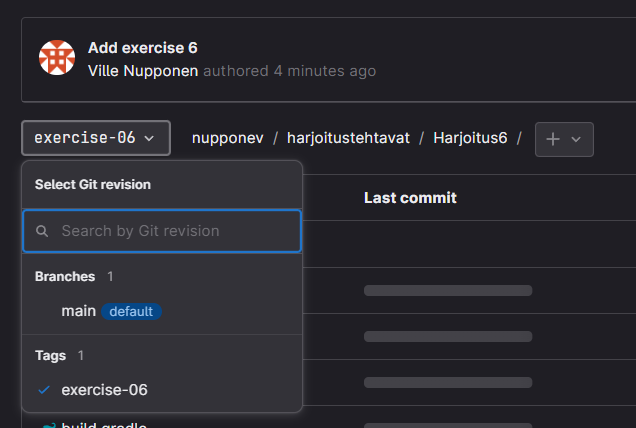
\includegraphics[width=0.8\textwidth]{figures/gitlab-change-branch-to-tag.png}
    \caption{Gitlabissa koodin näyttäminen tietyn tagin mukaan}
    \label{fig:gitlab-change-branch-to-tag}
\end{figure}

Harjoitus 7 olettaa ilmeisesti, että edellisellä harjoituksessa ei olisi
käytetty Composea vaan tehty perinteisillä View komponenteilla. Lähin vastine
Composen kanssa lienee se, että teen oman Composablen. Lisäksi harjoituksessa
ohjeistettu käyttämään RecyclerView-ominaisuutta, jolle hyvä vastine Composen
puolella on LazyColumn, joka oli jo käytössä.

Varsinaisen koodin muuttamiseen ei mene minuuttia kauempaa, mutta ilmeisesti
nyt tuli vastaan mahdollisesti ensimmäinen ongelma bind mountin kanssa. Eri
tiedostojärjestelmät ilmeisesti huomioivat kirjainkoon erilailla. Tämän
seurauksena onnistuin lisäämään harjoitus6:n versionhallintaan kahdesti. Toinen
kansio alkoi isolla kirjaimella ja toinen pienellä. Muutokset olin tietysti
ehtinyt jo pushata ja suoraan main-branchiin, joten historian korjaus ei
onnistu branchin suojauksen vuoksi. Uutta committia siis perään, jossa
poistettu duplikaatti. Asiaa toki hiukan hankaloitti se ettei tiedostoissa ne
näkynyt kahtena vaan ainoastaan git tunnisti ne erillisiksi. Sen tarkmmin
perehtymättä ongelma korjattu, muutokset tehty uudelleen ja testattu.

\section{Harjoitus 8}

Tässä harjoituksessa lisätään mahdollisuus järjestää sijainnin aikaleiman
mukaan, joko laskevaan tai nousevaan järjestykseen. Järjestys tallennetaan,
jotta järjestys on seuraavalla sovelluksen käyttökerralla sama eikä nollaannu
joka kerta kun sovelluksen avaa uudelleen. Toteutetaan lisäksi mahdollisuus
poistaa tallennettuja sijainteja.

Käyttäjän preferenceistä saadaan tehtyä käytevästi oma repository, ja sen myötä
ketjujettua Flow peräkkäin. Toki tässä tapauksessa halutaan saada myös
ensimmäinen tieto UiState:lle, joten sisäkkäin laittaminen auttaa siinä, kuten
koodissa \ref{lst:chain-flows} on tehty. Esimerkkejä ketjutuksee ja sisäkkäin
laittamiseen on saatu blogipostista \parencite{KotlinFlowNestingVSChaining}.

\begin{lstlisting}[
    basicstyle=\small,
    label={lst:nested-flows},
    caption={Useamman flown käyttäminen yhdessä},
    language=Kotlin,
]
@OptIn(FlowPreview::class)
val locationUiState: StateFlow<LocationUiState> =
    userPreferencesRepository.isAscOrder
        .flatMapMerge { isAscOrder ->
            (if (isAscOrder) locationRepository.getAllOrderByTimestampAsc()
            else locationRepository.getAllOrderByTimestampDesc())
                .map { locations ->
                    LocationUiState(locations = locations, isAscOrder = true)
                }
        }
        .stateIn(
            scope = viewModelScope,
            started = SharingStarted.WhileSubscribed(TIMEOUT_MILLIS),
            initialValue = LocationUiState()
        )
\end{lstlisting}

Jotta UI saadaan hiukan ''eloisammaksi'' niin laitetaan järjestyksen
vaihtopainikkeeseen hiukan animointia niin pääsee niitäkin testaamaan tässä
samalla. Animaatioiden tekemisen tueksi löytyi hyvä blogi postaus
\parencite{CardFlipAnimationWithJetpackCompose}.

Emulattorista löytyy kätevä screen recorder, jolla saadaan nauhoitettua
animaatiota. Videon laittaminen kuitenkin tähän dokumenttiin on jokseenkin
haastavaa, joten on se saatavilla Oppimispäiväkirja repositoryssa other
-kansiossa.

Merkittäviä ongelmia järjestämisessä ei tule, kunhan animaatioon laittaa oikean
luvun eikä vahingossa kymmenkertaista (nollan 180f vs 1800f) niin ei iconi
kierry liian montaa kertaa X-akselin ympäri. Lisäksi hyvä olla tarkkana
kopioinnissa ettei jätä molempiin tietokantakyseyihin järjestykseksi DESC, kun
silloin ei oikein järjestys vaihdu vaikka painike toimiikin.

% TODO: poistaminen

Vaikutteita tähän ja jonkin verran myös harjoituksiin 6 ja 7 se on tullut
''Now In Android''-esimerkistä \parencite{GithubAndroidNowInAndroid}. Lisäksi
Prefence DataStoren käyttämiseen käytetty tukena ''Dessert Release App''
-harjoitusta \parencite{GithubGoogleDevTrainingDessertRelease}.

\section{Tuntikirjanpito}

Oheiseen talukkoon on koottu harjoitustehtäviin käytetyt tunnit.

\begin{table}[H]
  \centering
  \label{tab:other-studing-working-hours}
  \begin{tabular*}{\linewidth}{@{\extracolsep{\fill}} l c c c r }
    \textbf{Tekeminen} & \textbf{Päivämäärä} & \textbf{Aloitettu} & \textbf{Lopetettu} & \textbf{Määrä} \\
    \hline
    Harjoitus 2  & 23.05.2023 & 05:15 & 05:25 &    10m \\
    Harjoitus 3  & 23.05.2023 & 05:25 & 08:05 & 2h 40m \\
    Harjoitus 3  & 24.05.2023 & 06:15 & 06:30 &    15m \\
    Harjoitus 4  & 24.05.2023 & 06:30 & 08:40 & 2h 10m \\
    Harjoitus 5  & 24.05.2023 & 08:50 & 09:05 &    15m \\
    Harjoitus 5  & 24.05.2023 & 09:25 & 12:55 & 3h 30m \\
    Harjoitus 6  & 24.05.2023 & 16:30 & 19:40 & 3h 10m \\
    Harjoitus 6  & 25.05.2023 & 06:40 & 08:30 & 1h 50m \\
    Harjoitus 7  & 25.05.2023 & 08:30 & 09:10 &    40m \\
    Harjoitus 8  & 25.05.2023 & 12:35 & 15:30 & 2h 55m \\
    Harjoitus 8  & 26.05.2023 & 08:30 & 08:45 &    15m \\
    \hline
    \multicolumn{4}{l}{\textbf{Yhteensä}} & \textbf{XXh XXm} \\
  \end{tabular*}
\end{table}


\chapter{PROJEKTI}
\label{ch:projekti}
Tähän tulee tietoa projektin tekemisestä

Android Studio templatet päivitty:
% https://developer.android.com/studio/releases#updates-to-npw-nmw

Kotlin 1.9.0 toimii! Ts. kotlinCompilerExtensionVersion '1.5.0' toimii, joten voi käyttää kotlin 1.9.0.

Navigaatio ohjeita:
% https://developer.android.com/codelabs/basic-android-kotlin-compose-navigation?hl=en#3

Esimerkkejä:
% https://github.com/android/compose-samples/tree/main

Kehittäjätilin luonti Google Play Consolee > sivuston vahvistaminen > DNS siirto

% https://stackoverflow.com/a/50361633/8380119

Bundler: sass-embedded-1.64.1-x86_64-linux-musl requires ruby version >= 3.0.0, which is incompatible with the current version, ruby 2.7.4p191


\begin{table}[H]
    \centering
    \label{tab:android-basics-with-compose-working-hours}
    \begin{tabular*}{\linewidth}{@{\extracolsep{\fill}} l c c c r }
        \textbf{Päivämäärä} & \textbf{Aloitettu} & \textbf{Lopetettu} & \textbf{Määrä} \\
        \hline
        25.07.2023 & 06:40 & 11:40 & 5h 00m \\
        25.07.2023 & 12:00 & 12:20 &    20m \\
        25.07.2023 & 15:15 & 17:30 & 2h 15m \\
        26.07.2023 & 08:20 & 10:30 & 2h 10m \\
        26.07.2023 & 10:50 & 11:30 &    40m \\
        26.07.2023 & 13:00 & 21:10 & 7h 10m \\
        27.07.2023 & 10:25 & 10:35 &    10m \\
        \hline
        \multicolumn{3}{l}{\textbf{Yhteensä}} & \textbf{XXh XXm} \\
    \end{tabular*}
\end{table}


\chapter{YHTEENVETO}
\label{ch:yhteenveto}
Kurssin suoritus on mahdollisesti jokseenkin vajaavainen ja ei lähelläkään sitä
miihen olisi voinut pystyä mikäli ajanhallinta olisi vain ollut kunnossa.
Kurssin toteuttaminen muutaman päivän ryppäinä useiden viikkojen tai jopa
kuukausien tauolla aiheutti jonkin verran ylimääräistä työtä, mutta asioiden
ollessa muuten melko yksinkertaisia, nopealla vilkaisulla pääsi jälleen
kärrylle.

Opiskelussa käytetyt kurssit toivat hyvin asioita esille ja olivat mukavan
yksinkertaisia ja kevyitä tehdä. Lähes 10 vuoden ohjelmointiosaamisen ansioista
asioiden oppiminen onnistui lisäksi pitkälti ongelmitta. Kehittämisessä on
lisäksi selvästi nähtävissä ero siihen, mitä kehittäminen oli vuonna 2013 kun
tehtiin Microsoft Phonelle.

Laaja harjoitustyö on selvästi keskeneräinen ja kehitys tulee jatkumaan aina
kun löytyy vapaata aikaa ja innostusta. Projektiin on jo mahdollisesti löytynyt
graaffikkokin niin saa huomattavasti näyttävämpää jälkelä kuin itse nopeasti
AI:n avustuksella. Tavoitteena on päästä testaamaan sovellusta seuraavalla
leirillä jolla osallistun kun sovellus on hiukan liian vajaavainen, että olisi
voinut testata leirillä, jolla olen parhaillaan tätä yhteenvetoa kirjoittaessa.


%%%%% Bibliography/references.

% Print the bibliography according to the
% information in ./tex/references.bib and
% the in-line citations used in the body of
% the thesis.
% \emergencystretch=2em
\printbibliography[heading=bibintoc]

%%%%% Appendices.

% Use only if it clarifies the structure of
% the document. Remember to introduce each
% appendix and its content.

\begin{appendices}

\chapter{Esimerkki liite}
\label{ch:example-appendix}
\begin{lstlisting}[
    basicstyle=\small,
    label={lst:example-appendix},
    breaklines=true,
]
ESIMERKKI LIITE
\end{lstlisting}


\end{appendices}

\end{document}
